% OL (working name; "orientation likelihood ratio"): out-of-distribution detection with a frozen diffusion model from one number per U-Net
%   block, the amplitude a_h = mean over channels of log max over positions |h - spatial mean| of the block output at sigma_1 = 0.01, read
%   for the blocks up to A (the first decoder block with a 16x16 output; the pass stops there).  From held-out ID images (val1): the mean m
%   and covariance S of the profile, and m_o = the mean profile of the same images in the seven other orientations of the square.
%   Score = -(a - m*)^T (S + ridge)^-1 (a - m*), m* = m + c (m - m_o), c = 8: one Mahalanobis distance = the Gaussian log-likelihood ratio
%   between N(m, S) and N(m_o, (1 + 1/c) S).  Nothing trained by gradient descent, no further network, no human label, no OOD image.
%   26f WIP, Japanese; MIRU 2025 class.  Splits: train (not used by OL) / val1 / val2 (development) / test ... test6.
% build: python3 gen/ol_gen.py && python3 assemble.py && latexmk -r latexmkrc main.tex
% numbers: numbers_ol.tex and the tab_*_ol.tex and supp_*_ol.tex tables are written by gen/ol_gen.py from gen/data/ol
%   (server names of the splits: test2 = this paper's test, test3 ... test6 = test2 ... test5, test7 = test6; fresh = val2).
%   numbers_bench.tex supplies the timing of the published methods and the CFS reproduction.
\documentclass[MIRU,submit]{miru2025j}
\usepackage[dvipdfmx]{graphicx}
\usepackage[dvipdfmx,table]{xcolor}
\definecolor{firstblue}{RGB}{189,215,238}   % background of the cells where Ours ties or beats the best comparison method (light blue)
\definecolor{lossred}{RGB}{246,200,192}      % background of the losses in the per-pair tables (light red)
\definecolor{navyc}{RGB}{31,58,122}\definecolor{redc}{RGB}{192,57,43}   % Figure 1: the ID side (navy) and the test image / what is computed (red)
\usepackage{amsmath,amssymb}
\usepackage{booktabs}
\usepackage{adjustbox}
\usepackage{float}   % [H]: the tables of the supplement stay below their heading
\usepackage{array}
\usepackage{tikz}
\usetikzlibrary{arrows.meta,positioning,calc,fit,decorations.pathreplacing}
\usepackage{pgfplots}
\pgfplotsset{compat=1.16}
\makeatletter
\renewcommand{\signame}{26f WIP中間発表}   % running head (in place of the symposium name)
\renewcommand{\MIRUPreface}{}                        % removes the "CONFIDENTIAL ..." notice of the submission mode
\makeatother
\newcommand{\veps}{\vec{\varepsilon}}
\newcommand{\Vf}{\mathbf{V}}   % the upside-down flip is a matrix (bold), vectors carry arrows
\newcommand{\Ours}{OL}   % the name of the method (working name)
\newcommand{\Pm}{\mathbf{P}}\newcommand{\Gm}{\mathbf{G}}\newcommand{\vd}{\vec{\delta}}\newcommand{\vmu}{\vec{\mu}}\newcommand{\va}{\vec{a}}\newcommand{\Sm}{\mathbf{S}}\newcommand{\Id}{\mathbf{I}}
\makeatletter\newcommand{\inputrows}[1]{\@@input #1 }\makeatother   % primitive \input: a table body may then begin with a rule (\noalign)
\renewcommand{\eqref}[1]{(\ref{#1})}   % amsmath's \eqref puts extra space before the Japanese text that follows
\renewcommand{\dbltopfraction}{0.95}\renewcommand{\topfraction}{0.95}\renewcommand{\textfraction}{0.05}\renewcommand{\dblfloatpagefraction}{0.9}\setcounter{dbltopnumber}{3}\setcounter{topnumber}{3}
\renewcommand{\floatpagefraction}{0.9}
\makeatletter   % figures and tables over both columns: captions over the full width (the class narrows them to 2/3)
\renewenvironment{figure*}{\@floatenv\capwidth\textwidth\ecapwidth\textwidth\abovecaptionskip1mm\belowcaptionskip\z@\@dblfloat{figure}}{\end@dblfloat}
\renewenvironment{table*}{\@floatenv\capwidth\textwidth\ecapwidth\textwidth\abovecaptionskip\z@\belowcaptionskip1mm\@dblfloat{table}}{\end@dblfloat}
\renewenvironment{table}{\@floatenv\capwidth\columnwidth\ecapwidth\columnwidth\abovecaptionskip\z@\belowcaptionskip1mm\@float{table}}{\end@float}
\makeatother
% numbers_bench.tex -- the three numbers the resume takes from earlier measurements with the shared code base:
%   the timing session of the published methods (repetitions, CPU clock) and the largest difference of the CFS
%   reproduction from the published values.
\newcommand{\cpuReps}{15}
\newcommand{\cpuGHz}{2.30\,GHz}
\newcommand{\cfsRepMaxDiff}{0.5}
  % timing of the comparison methods, the CFS reproduction
% written by gen/ol_gen.py
\newcommand{\olTestOL}{95.6}
\newcommand{\olTestVf}{84.7}
\newcommand{\olSixMin}{95.3}
\newcommand{\olSixMax}{95.7}
\newcommand{\olSixMean}{95.5}
\newcommand{\olSixMeanB}{95.51}
\newcommand{\olSixVf}{84.8}
\newcommand{\olSixVfMin}{84.3}
\newcommand{\olSixVfMax}{85.1}
\newcommand{\olSixHf}{58.5}
\newcommand{\olSixFpr}{17.9}
\newcommand{\olSixAll}{95.4}
\newcommand{\olSixL}{94.4}
\newcommand{\olSixT}{87.5}
\newcommand{\olSixAllGap}{0.12}
\newcommand{\olSixLGap}{1.1}
\newcommand{\olSixTGap}{8.0}
\newcommand{\olSixCten}{95.1}
\newcommand{\olSixAllCten}{93.4}
\newcommand{\olSixLCten}{94.9}
\newcommand{\olSixTCten}{76.3}
\newcommand{\olSixVfCten}{88.4}
\newcommand{\olSixHfCten}{50.2}
\newcommand{\olSixMinCten}{94.2}
\newcommand{\olSixMaxCten}{95.8}
\newcommand{\olSixSVHN}{96.9}
\newcommand{\olSixAllSVHN}{99.5}
\newcommand{\olSixLSVHN}{95.2}
\newcommand{\olSixTSVHN}{90.6}
\newcommand{\olSixVfSVHN}{63.9}
\newcommand{\olSixHfSVHN}{68.2}
\newcommand{\olSixMinSVHN}{96.6}
\newcommand{\olSixMaxSVHN}{97.1}
\newcommand{\olSixCelebA}{100.0}
\newcommand{\olSixAllCelebA}{100.0}
\newcommand{\olSixLCelebA}{100.0}
\newcommand{\olSixTCelebA}{100.0}
\newcommand{\olSixVfCelebA}{99.9}
\newcommand{\olSixHfCelebA}{50.0}
\newcommand{\olSixMinCelebA}{99.9}
\newcommand{\olSixMaxCelebA}{100.0}
\newcommand{\olSixIN}{85.9}
\newcommand{\olSixAllIN}{84.3}
\newcommand{\olSixLIN}{82.3}
\newcommand{\olSixTIN}{73.1}
\newcommand{\olSixVfIN}{74.7}
\newcommand{\olSixHfIN}{50.2}
\newcommand{\olSixMinIN}{84.6}
\newcommand{\olSixMaxIN}{87.1}
\newcommand{\olSixFM}{99.7}
\newcommand{\olSixAllFM}{99.7}
\newcommand{\olSixLFM}{99.6}
\newcommand{\olSixTFM}{97.6}
\newcommand{\olSixVfFM}{97.1}
\newcommand{\olSixHfFM}{74.0}
\newcommand{\olSixMinFM}{99.4}
\newcommand{\olSixMaxFM}{99.8}
\newcommand{\olEqSix}{91.9}
\newcommand{\olEqSixMin}{91.6}
\newcommand{\olEqSixMax}{92.1}
\newcommand{\olEqSixDrop}{3.6}
\newcommand{\olEqSixVf}{80.6}
\newcommand{\olEqSixCten}{88.7}
\newcommand{\olEqSixDropCten}{6.4}
\newcommand{\olEqSixSVHN}{97.1}
\newcommand{\olEqSixDropSVHN}{-0.3}
\newcommand{\olEqSixCelebA}{100.0}
\newcommand{\olEqSixDropCelebA}{0.0}
\newcommand{\olEqSixIN}{74.7}
\newcommand{\olEqSixDropIN}{11.3}
\newcommand{\olEqSixFM}{99.0}
\newcommand{\olEqSixDropFM}{0.7}
\newcommand{\olNCten}{258}
\newcommand{\olNTex}{199}
\newcommand{\olNBlkCten}{23}
\newcommand{\olNRefMin}{1{,}500}
\newcommand{\olNRefMax}{2{,}000}
\newcommand{\olNStored}{552}
\newcommand{\olMBOurs}{0.0011}
\newcommand{\olDeltaMin}{0.9}
\newcommand{\olDeltaMax}{8.8}
\newcommand{\olNBlkMin}{8}
\newcommand{\olNBlkMax}{25}
\newcommand{\olDeltaCten}{1.8}
\newcommand{\olDeltaSVHN}{1.1}
\newcommand{\olDeltaCelebA}{8.8}
\newcommand{\olDeltaIN}{0.9}
\newcommand{\olDeltaFM}{2.8}
\newcommand{\olHrNCal}{??}
\newcommand{\olHrNBlk}{??}
\newcommand{\olSecOL}{0.068}
\newcommand{\olFwdAll}{0.180}
\newcommand{\olFwdA}{0.066}
\newcommand{\olFwdAShare}{37}
\newcommand{\olJudgeMs}{1.8}
\newcommand{\olSecCfs}{0.181}
\newcommand{\olSecCfsStop}{0.087}
\newcommand{\olSecCfsKnn}{0.185}
\newcommand{\olSecCfsKnnStop}{0.090}
\newcommand{\olSecRatioCfsKnn}{0.75}
\newcommand{\olSecRatioCfs}{0.79}
\newcommand{\olSecRatioCfsKnnFull}{0.37}
\newcommand{\olCpuHere}{Intel Core i9-7920X, 2.90\,GHz}
\newcommand{\olPairs}{51}
\newcommand{\olNPrior}{10}
\newcommand{\olNStat}{8}
\newcommand{\olBestPriorName}{CFSの kNN ヘッド}
\newcommand{\olBestPriorMean}{88.0}
\newcommand{\olGapCfsKnn}{7.6}
\newcommand{\olGapCfsKnnLo}{7.0}
\newcommand{\olGapCfsKnnHi}{8.3}
\newcommand{\olGapCfs}{10.0}
\newcommand{\olGapCfsLo}{9.3}
\newcommand{\olGapCfsHi}{10.7}
\newcommand{\olCfsMean}{85.6}
\newcommand{\olVfBestPriorName}{EigenScore}
\newcommand{\olVfBestPriorAvg}{78.6}
\newcommand{\olPriorBestCten}{85.4}
\newcommand{\olPriorBestCtenName}{CFSの kNN ヘッド}
\newcommand{\olTestCten}{95.6}
\newcommand{\olPriorBestGapCten}{$+$10.2}
\newcommand{\olGapCfsKnnCten}{$+$10.2}
\newcommand{\olVerdictCfsKnnCten}{win}
\newcommand{\olPriorBestSVHN}{99.8}
\newcommand{\olPriorBestSVHNName}{DiffPath}
\newcommand{\olTestSVHN}{96.9}
\newcommand{\olPriorBestGapSVHN}{$-$2.9}
\newcommand{\olGapCfsKnnSVHN}{$+$3.2}
\newcommand{\olVerdictCfsKnnSVHN}{win}
\newcommand{\olPriorBestCelebA}{99.8}
\newcommand{\olPriorBestCelebAName}{DiffPath}
\newcommand{\olTestCelebA}{100.0}
\newcommand{\olPriorBestGapCelebA}{$+$0.2}
\newcommand{\olGapCfsKnnCelebA}{$+$0.4}
\newcommand{\olVerdictCfsKnnCelebA}{win}
\newcommand{\olPriorBestIN}{65.5}
\newcommand{\olPriorBestINName}{CFS}
\newcommand{\olTestIN}{85.8}
\newcommand{\olPriorBestGapIN}{$+$20.3}
\newcommand{\olGapCfsKnnIN}{$+$24.4}
\newcommand{\olVerdictCfsKnnIN}{win}
\newcommand{\olPriorBestFM}{99.8}
\newcommand{\olPriorBestFMName}{CFSの kNN ヘッド}
\newcommand{\olTestFM}{99.8}
\newcommand{\olPriorBestGapFM}{$+$0.0}
\newcommand{\olGapCfsKnnFM}{$+$0.0}
\newcommand{\olVerdictCfsKnnFM}{tie}
\newcommand{\olPriorWinMin}{34}
\newcommand{\olPriorWinMax}{50}
\newcommand{\olWtlCfsKnn}{37/14/0}
\newcommand{\olWtlCfs}{42/9/0}
\newcommand{\olPriorLossMax}{10}
\newcommand{\olPriorLossMaxName}{MSMA型, DiffPath}
\newcommand{\olNLostPrior}{11}
\newcommand{\olNLostPriorSVHN}{11}
\newcommand{\olNLostPriorVf}{1}
\newcommand{\olLostPriorList}{SVHNの上下反転(EigenScore), SVHNを分布内とするCIFAR-10(NLL・TT・MSMA型・DiffPath), SVHNを分布内とするCIFAR-100(NLL・TT・MSMA型・DiffPath), SVHNを分布内とするCelebA(NLL・TT・MSMA型・DiffPath), SVHNを分布内とするTextures(MSMA型・DiffPath), SVHNを分布内とするTiny-ImageNet(NLL・TT・MSMA型・DiffPath), SVHNを分布内とするLSUN(NLL・IC-PNG・TT・MSMA型・DiffPath), SVHNを分布内とするImageNet(NLL・TT・MSMA型・DiffPath), SVHNを分布内とするImageNet32(NLL・IC-PNG・TT・MSMA型・DiffPath), SVHNを分布内とするPlaces365(NLL・TT・MSMA型・DiffPath), SVHNを分布内とする一様ノイズ(NLL・IC-PNG・IC-J2K・TT・MSMA型・DiffPath)}
\newcommand{\olOursColsBest}{6}
\newcommand{\olUnderlineNote}{}
\newcommand{\olTestSVHNBehind}{2.9}
\newcommand{\olTestFMBehind}{0.0}
\newcommand{\olNImgCfs}{50{,}000}
\newcommand{\olMBCfsKnn}{102}
\newcommand{\olImgRatio}{25}
\newcommand{\olEqOL}{92.0}
\newcommand{\olEqCfs}{82.5}
\newcommand{\olEqCfsKnn}{84.4}
\newcommand{\olOrigCfs}{85.6}
\newcommand{\olOrigCfsKnn}{88.0}
\newcommand{\olEqDropOL}{3.6}
\newcommand{\olEqDropCfs}{3.2}
\newcommand{\olEqDropCfsKnn}{3.6}
\newcommand{\olEqGapCfsKnn}{7.6}
\newcommand{\olEqGapCfsKnnLo}{6.9}
\newcommand{\olEqGapCfsKnnHi}{8.4}
\newcommand{\olEqGapCfs}{9.6}
\newcommand{\olEqGapCfsLo}{8.7}
\newcommand{\olEqGapCfsHi}{10.4}
\newcommand{\olOrigGapCfsKnnB}{7.6}
\newcommand{\olOrigGapCfsKnnBLo}{7.0}
\newcommand{\olOrigGapCfsKnnBHi}{8.3}
\newcommand{\olEqWtlCfsKnn}{36/3/4}
\newcommand{\olEqWtlCfs}{43/0/0}
\newcommand{\olEqNPairs}{43}
\newcommand{\olOrigWtlCfsKnnB}{35/8/0}
\newcommand{\olEqNLostCfsKnn}{4}
\newcommand{\olEqLostCfsKnnList}{FashionMNISTを分布内とするMNIST, FashionMNISTを分布内とするKMNIST, FashionMNISTを分布内とするOmniglot, FashionMNISTを分布内とするnotMNIST}
\newcommand{\olEqGapCfsKnnCten}{$+$13.5}
\newcommand{\olEqOLCten}{88.9}
\newcommand{\olEqCfsKnnCten}{75.4}
\newcommand{\olEqGapCfsKnnSVHN}{$+$3.6}
\newcommand{\olEqOLSVHN}{97.3}
\newcommand{\olEqCfsKnnSVHN}{93.6}
\newcommand{\olEqGapCfsKnnCelebA}{$+$0.3}
\newcommand{\olEqOLCelebA}{100.0}
\newcommand{\olEqCfsKnnCelebA}{99.7}
\newcommand{\olEqGapCfsKnnIN}{$+$21.6}
\newcommand{\olEqOLIN}{75.0}
\newcommand{\olEqCfsKnnIN}{53.4}
\newcommand{\olEqGapCfsKnnFM}{$-$1.0}
\newcommand{\olEqOLFM}{98.9}
\newcommand{\olEqCfsKnnFM}{99.9}
\newcommand{\olTestFpr}{18.6}
\newcommand{\olCfsKnnFpr}{35.9}
\newcommand{\olCfsFpr}{45.5}
\newcommand{\olEqVfOL}{80.3}
\newcommand{\olEqVfCfsKnn}{72.3}
\newcommand{\olCfsValMean}{86.8}
\newcommand{\olCfsKnnValMean}{88.1}
\newcommand{\olGapCfsKnnVal}{7.6}
\newcommand{\olDqOLMin}{62.7}
\newcommand{\olDqOLMax}{90.0}
\newcommand{\olDqOLMean}{76.5}
\newcommand{\olDqCfsKnnMin}{64.0}
\newcommand{\olDqCfsKnnMax}{88.7}
\newcommand{\olDqCfsKnnMean}{74.5}
\newcommand{\olDqCfsMin}{57.4}
\newcommand{\olDqCfsMax}{88.9}
\newcommand{\olDqCfsMean}{72.8}
\newcommand{\olDqLMin}{58.7}
\newcommand{\olDqLMax}{81.4}
\newcommand{\olDqLMean}{70.1}
\newcommand{\olDqTMin}{66.2}
\newcommand{\olDqTMax}{91.6}
\newcommand{\olDqTMean}{78.4}
\newcommand{\olDqNHigher}{5}
\newcommand{\olDqSVHNMax}{66.5}
\newcommand{\olDqINJpeg}{98.5}
\newcommand{\olDqCfsKnnINJpeg}{71.0}
\newcommand{\olDqBlurOL}{90.0}
\newcommand{\olDqBlurCfsKnn}{88.7}
\newcommand{\olDqBlurHalfOL}{62.7}
\newcommand{\olDqJpegOL}{69.0}
\newcommand{\olDqJpegCfsKnn}{64.7}
\newcommand{\olVarTrained}{95.5}
\newcommand{\olVarRinit}{72.0}
\newcommand{\olVarRshuf}{67.9}
\newcommand{\olVarRinitVf}{55.3}
\newcommand{\olVarRshufVf}{56.9}
\newcommand{\olVarTrainedVf}{85.0}
\newcommand{\olVarBy}{84.2}
\newcommand{\olVarByTrained}{97.0}
\newcommand{\olVarByL}{64.1}
\newcommand{\olVarByT}{84.9}
\newcommand{\olVarByVf}{59.4}
\newcommand{\olVarNBy}{6}
\newcommand{\olVarByMin}{60.0}
\newcommand{\olVarByMax}{99.4}
\newcommand{\olVarRinitL}{57.9}
\newcommand{\olVarRinitT}{73.1}
\newcommand{\olVarTrainedL}{94.5}
\newcommand{\olVarTrainedT}{87.3}
\newcommand{\olVarRinitCten}{65.4}
\newcommand{\olVarRshufCten}{62.3}
\newcommand{\olVarRinitSVHN}{74.8}
\newcommand{\olVarRshufSVHN}{70.7}
\newcommand{\olVarRinitCelebA}{77.0}
\newcommand{\olVarRshufCelebA}{76.4}
\newcommand{\olVarRinitIN}{60.7}
\newcommand{\olVarRshufIN}{60.2}
\newcommand{\olVarRinitFM}{81.8}
\newcommand{\olVarRshufFM}{69.9}
\newcommand{\olDevCzero}{87.8}
\newcommand{\olDevEqCzero}{83.2}
\newcommand{\olDevCone}{91.9}
\newcommand{\olDevEqCone}{86.8}
\newcommand{\olDevCfour}{94.9}
\newcommand{\olDevEqCfour}{90.6}
\newcommand{\olDevCeight}{95.6}
\newcommand{\olDevEqCeight}{91.8}
\newcommand{\olDevCsixteen}{95.6}
\newcommand{\olDevEqCsixteen}{92.0}
\newcommand{\olDevCsixtyfour}{95.0}
\newcommand{\olDevEqCsixtyfour}{91.0}
\newcommand{\olDevCinf}{94.5}
\newcommand{\olDevEqCinf}{90.1}
\newcommand{\olDevOv}{95.3}
\newcommand{\olDevEqOv}{91.3}
\newcommand{\olDevOnomirror}{95.6}
\newcommand{\olDevEqOnomirror}{91.9}
\newcommand{\olDevOquarter}{95.5}
\newcommand{\olDevEqOquarter}{91.6}
\newcommand{\olDevOflips}{95.0}
\newcommand{\olDevEqOflips}{90.9}
\newcommand{\olDevNfifty}{93.3}
\newcommand{\olDevEqNfifty}{88.4}
\newcommand{\olDevNhundred}{93.8}
\newcommand{\olDevEqNhundred}{89.7}
\newcommand{\olDevNfivehundred}{94.9}
\newcommand{\olDevEqNfivehundred}{90.8}
\newcommand{\olDevNthousand}{95.6}
\newcommand{\olDevEqNthousand}{91.5}
\newcommand{\olDevAll}{95.3}
\newcommand{\olDevEqAll}{90.9}
\newcommand{\olDevLstd}{95.2}
\newcommand{\olDevEqLstd}{91.2}
\newcommand{\olDevPk}{94.5}
\newcommand{\olDevEqPk}{90.2}
\newcommand{\olDevPkd}{91.2}
\newcommand{\olDevEqPkd}{86.1}
\newcommand{\olDevPkds}{91.2}
\newcommand{\olDevEqPkds}{85.7}
\newcommand{\olDevVfCeight}{85.2}
\newcommand{\olDevVfCinf}{87.0}
\newcommand{\olDevVfPk}{87.2}
\newcommand{\olDevSVHNOv}{96.0}
\newcommand{\olDevSVHNOquarter}{97.3}
\newcommand{\olDevCeightB}{95.55}
\newcommand{\olDevEqCeightB}{91.77}
\newcommand{\olDevSVHNAll}{99.5}
\newcommand{\olDevSVHNCeight}{97.3}
\newcommand{\olNDev}{62}
\newcommand{\olDevSeeds}{95.54, 95.55, 95.56}
\newcommand{\olDevSeedsEq}{91.66, 91.88, 91.78}
\newcommand{\olDevCutMin}{83}
\newcommand{\olDevCutMax}{85}
\newcommand{\olOracleCosMin}{0.72}
\newcommand{\olOracleCosMax}{0.86}
\newcommand{\olBarNat}{95.07}
\newcommand{\olBarEq}{90.33}
\newcommand{\olDevDiff}{0.003}
\newcommand{\olOraclePool}{97.3}
\newcommand{\olOracleSet}{98.4}
\newcommand{\olOracleGap}{1.7}
\newcommand{\olDevSeedZero}{95.5}
\newcommand{\olOraclePoolCten}{96.8}
\newcommand{\olOraclePoolIN}{89.9}
\newcommand{\olOracleSsb}{86.0}
\newcommand{\olOracleCHundred}{91.8}
\newcommand{\olDevCHundred}{89.7}
\newcommand{\olDevSsb}{64.6}
     % gen/ol_gen.py
\usepackage{etoolbox}
\makeatletter
\patchcmd{\@makecaption}{\vskip-1.5mm}{\vskip0.3mm}{}{\PackageError{main}{makecaption not patched}{}}   % multi-line table captions no longer touch the top rule
\setlength{\@fptop}{0pt}\setlength{\@fpbot}{0pt plus 1fil}   % pages that hold only floats start at the top instead of centring them
\makeatother
\hyphenation{FashionMNIST ImageNet EigenScore DiffPath}   % no hyphenation of these names inside the Japanese text
\raggedbottom
\begin{document}
\title{\begin{tabular}[c]{@{}c@{}}\textbf{OOD Detection by an Orientation Likelihood Ratio}\end{tabular}}
\affiliate{sfc}{慶應義塾大学 総合政策学部B3 中澤・大越研究室 d-hacks}
\affiliate{sfc2}{慶應義塾大学大学院 政策・メディア研究科}
\author{omote}{}{sfc}[]
\author{親:zackeyさん}{}{sfc2}[]
\maketitle

\section*{概要}
凍結した拡散モデルによる分布外検知では, 1回の順伝播で中間特徴を読むCFSが最良であるが, 1{,}024次元の特徴を学習画像5万枚と比べる. 本研究の\Ours{}は, U-Netのブロックごとに数値を1つ(振幅)だけ読み,その並びを1つの式で判定する. 分布内の画像\olNRefMax{}枚の並びの平均と共分散,同じ画像を残り7つの向き(反転と回転)にしたときの並びの平均を求める. スコアは,分布内の平均を,向きを変えた平均の反対側へ動かした点へのマハラノビス距離で, 2つの正規分布の対数尤度比に等しい. 勾配による学習,追加のネットワーク,人手のラベル,分布外の画像は使わない. 5つの分布内データセットで,自然画像の分布外集合に対する平均AUROCは\olTestOL\%で,先行研究の最良(CFS)を\olGapCfsKnn{}ポイント上回った(95\%信頼区間[\olGapCfsKnnLo, \olGapCfsKnnHi]). 6つのテスト分割では\olSixMin{}〜\olSixMax\%であった. 順伝播は途中で止める1回で, CPU時間はCFSの\olSecRatioCfsKnn{}倍である. 縮小の履歴をそろえた対照でも差は保たれた. 定数1つは開発用の分割で決め,テスト分割は以前に他の手法で結果を見たものである.
\section{はじめに}
拡散モデル~\cite{song2021score,karras2022edm}は,生成のために学習したモデルを凍結したまま分布外検知に使える. 尤度や統計量による検知~\cite{serra2020input,mahmood2021msma,heng2024diffpath,alexis2026gepc,shoushtari2026eigenscore}は, 1枚あたり10回から数百回のネットワークの評価を要する. CFS~\cite{rouzoumka2026cfs}は,低いノイズで1回通したときの中間特徴~\cite{xiang2023ddae}を使い, 1回の順伝播でこれらを上回る.

\begin{figure*}[t]\centering
\begin{adjustbox}{max width=\textwidth}% fig_method.tex -- Figure 1: the method in pictures (TikZ, drawn by hand; absolute coordinates in cm, natural width about 18.7 cm).
%   (a) test time: the image goes through the frozen U-Net up to block A (the pass stops there); of every block ONE number is read (the
%       amplitude: per channel the largest deviation from the spatial mean, log, mean over channels).  The numbers form the profile.  The
%       score is one Mahalanobis distance: from the profile to the point mu*.
%   (b) once, before: the n held-out ID images in the eight orientations of the square.  As they are: mean mu and covariance S of the
%       profile.  The seven other orientations: the mean mu_o.  No feature of a training image is stored.
%   (c) what the score means: mu* is mu moved away from mu_o; a profile on the mu_o side is far from mu*.
%   Colours: black, navy (ID side), red (the test image / what is computed).  The curves and the layout of (c) are a schematic, not data.
\begin{tikzpicture}[font=\scriptsize, >={Stealth[length=1.5mm, width=1.2mm]}, line join=round, line cap=round,
  lab/.style={font=\tiny, inner sep=1pt, align=center}, ttl/.style={font=\scriptsize, anchor=south west, inner sep=0pt}]
\def\unet#1#2#3#4#5{% origin (left block, centre height), scale, style of the down path and bottom, style of block A, style of the rest of the up path
  \begin{scope}[shift={#1}, scale=#2]
    \foreach \dx/\yc/\h in {0/0/1.5, 0.3/0/1.5, 0.75/-0.5/1.0, 1.05/-0.5/1.0, 1.5/-0.95/0.6, 1.8/-0.95/0.6, 2.25/-0.95/0.6, 2.55/-0.95/0.6}
      \draw[#3] (\dx,\yc-\h/2) rectangle ++(0.22,\h);
    \draw[#4] (3.2,-1.0) rectangle ++(0.22,1.0);
    \foreach \dx/\yc/\h in {3.5/-0.5/1.0, 3.95/0/1.5, 4.25/0/1.5}
      \draw[#5] (\dx,\yc-\h/2) rectangle ++(0.22,\h);
    \draw[#3] (0.52,0) -- (0.75,-0.5) (1.27,-0.5) -- (1.5,-0.95) (2.02,-0.95) -- (2.25,-0.95) (2.77,-0.95) -- (3.2,-0.5);
    \draw[#5] (3.72,-0.5) -- (3.95,0);
  \end{scope}}
%% ================================================================ (a) test time
\node[ttl] at (0,0.3) {\textbf{(a)}\ テスト時：ブロックAまで通し,ブロックごとに数値を1つだけ読む};
\node[inner sep=0, draw=black!60] at (0.62,-1.0) {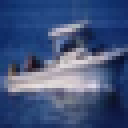
\includegraphics[width=1.0cm]{figs/ex_id.png}};
\node[lab, anchor=north] at (0.62,-1.57) {テスト画像 $\vec{x}$};
\draw[->] (1.16,-1.0) -- node[above, lab] {$+\sigma_1\veps$} (1.84,-1.0);
\unet{(1.9,-1.0)}{1}{black, line width=0.7pt}{redc, fill=redc!35, line width=0.9pt}{black!40, densely dashed, line width=0.5pt}
\node[lab, anchor=south west] at (1.9,-0.2) {ノイズ除去器(U-Net, 凍結). 順伝播は1回};
\node[lab, anchor=north west, text=redc] at (5.02,-2.03) {\textbf{ブロックA}で止める};
\draw[black!70, decorate, decoration={brace, mirror, amplitude=3pt}] (1.9,-2.42) -- (5.32,-2.42);
\node[lab, anchor=north] at (3.6,-2.55) {ブロックAまでの出力};
% ---- the amplitude of one block: one channel, the largest deviation from its spatial mean
\draw[->] (6.5,-1.0) -- (7.2,-1.0);
\foreach \i/\j/\s in {0/0/12,1/0/20,2/0/8,3/0/15,4/0/10, 0/1/18,1/1/10,2/1/25,3/1/12,4/1/8, 0/2/8,1/2/15,2/2/12,3/2/90,4/2/20, 0/3/14,1/3/8,2/3/18,3/3/22,4/3/10, 0/4/10,1/4/16,2/4/9,3/4/13,4/4/17}
  \fill[black!\s] ({7.3+0.26*\i},{-0.55-0.26*\j}) rectangle ++(0.26,-0.26);
\draw[black!60] (7.3,-0.55) rectangle (8.6,-1.85);
\draw[redc, line width=1.0pt] (8.08,-1.07) rectangle ++(0.26,-0.26);
\node[lab, anchor=south] at (7.95,-0.52) {ブロック $h$ の1チャネル};
\node[lab, anchor=north, text=redc] at (7.95,-1.88) {平均から最も離れた値};
\node[lab, anchor=north] at (7.95,-2.2) {その大きさの対数を\\チャネルで平均};
\draw[->] (8.7,-1.2) -- node[above, lab] {$a_h(\vec{x})$} node[below, lab] {数値1つ} (9.75,-1.2);
% ---- the profile: one number per block up to A
\draw[black!45, rounded corners=3pt] (9.8,-0.2) rectangle (14.25,-3.15);
\draw[->, black!80] (10.25,-2.8) -- (14.1,-2.8); \draw[->, black!80] (10.25,-2.8) -- (10.25,-0.4);
\node[lab, anchor=north east] at (14.15,-2.84) {ブロック $h$};
\node[lab, anchor=south west] at (10.3,-0.62) {振幅 $a_h$};
\fill[navyc!18] (10.5,-1.75) -- (11.0,-1.45) -- (11.5,-1.6) -- (12.0,-1.25) -- (12.5,-1.0) -- (13.0,-1.35) -- (13.5,-1.15) -- (13.95,-1.45)
  -- (13.95,-1.95) -- (13.5,-1.65) -- (13.0,-1.85) -- (12.5,-1.5) -- (12.0,-1.75) -- (11.5,-2.1) -- (11.0,-1.95) -- (10.5,-2.25) -- cycle;
\draw[navyc, line width=0.9pt] (10.5,-2.0) -- (11.0,-1.7) -- (11.5,-1.85) -- (12.0,-1.5) -- (12.5,-1.25) -- (13.0,-1.6) -- (13.5,-1.4) -- (13.95,-1.7);
\draw[black, densely dashed, line width=0.8pt] (10.5,-1.75) -- (11.0,-1.4) -- (11.5,-1.5) -- (12.0,-1.05) -- (12.5,-0.75) -- (13.0,-1.15) -- (13.5,-0.9) -- (13.95,-1.15);
\draw[redc, line width=1.0pt] (10.5,-2.2) -- (11.0,-2.05) -- (11.5,-2.4) -- (12.0,-2.0) -- (12.5,-2.1) -- (13.0,-1.95) -- (13.5,-2.25) -- (13.95,-2.3);
\foreach \p in {(10.5,-2.2),(11.0,-2.05),(11.5,-2.4),(12.0,-2.0),(12.5,-2.1),(13.0,-1.95),(13.5,-2.25),(13.95,-2.3)} \fill[redc] \p circle (0.05);
\node[lab, anchor=south, text=redc] at (13.95,-0.75) {A};
\draw[black!55, densely dotted] (13.95,-2.8) -- (13.95,-0.78);
\node[lab, anchor=west] at (10.42,-0.95) {$\vmu^{*}$(破線)};
\node[lab, anchor=west, text=navyc] at (11.75,-0.62) {分布内の画像($\vmu$ と幅)};
\node[lab, anchor=west, text=redc] at (10.42,-2.62) {テスト画像 $\va(\vec{x})$};
\draw[<->, redc, line width=0.5pt] (12.5,-0.8) -- (12.5,-2.05);
% ---- one distance -> the score
\draw[->] (14.35,-1.6) -- (14.85,-1.6);
\node[draw=black, rounded corners=2pt, line width=0.9pt, inner sep=3pt, align=center, font=\tiny, text width=20mm] at (16.1,-1.6) {$\vmu^{*}$ までの\\マハラノビス距離\\(式は1つ)};
\draw[->] (17.3,-1.6) -- (17.75,-1.6);
\node[lab, anchor=west] at (17.72,-1.6) {$s(\vec{x})$};
\node[lab, anchor=north, text=black!60] at (16.1,-2.3) {近いほど分布内};
%% ================================================================ (b) prepared once
\node[ttl] at (0,-3.95) {\textbf{(b)}\ 事前の準備(1回だけ)：分布内の画像\olNRefMax{}枚を8つの向きで通す};
\node[inner sep=0, draw=navyc, line width=0.8pt] at (0.5,-5.0) {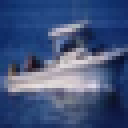
\includegraphics[width=0.62cm]{figs/ex_id.png}};
\node[lab, anchor=north, text=navyc] at (0.5,-5.36) {そのまま};
\foreach \x/\y/\r/\sx/\sy in {1.55/-4.72/0/1/-1, 2.3/-4.72/0/-1/1, 3.05/-4.72/180/1/1, 3.8/-4.72/90/1/1, 1.55/-5.52/270/1/1, 2.3/-5.52/90/1/-1, 3.05/-5.52/270/1/-1}
  \node[inner sep=0, rotate=\r, xscale=\sx, yscale=\sy] at (\x,\y) {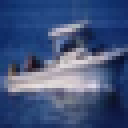
\includegraphics[width=0.62cm]{figs/ex_id.png}};
\node[lab, anchor=west] at (3.45,-5.52) {残り7つの向き};
\draw[->] (4.7,-5.1) -- (5.15,-5.1);
\unet{(5.25,-4.95)}{0.3}{black, line width=0.35pt}{redc, fill=redc!35, line width=0.35pt}{black!40, densely dashed, line width=0.3pt}
\draw[->] (6.7,-5.1) -- (7.15,-5.1);
\pgfmathsetseed{7}
\foreach \i in {1,...,12} {\pgfmathsetmacro{\sa}{0.2*(rnd-0.5)}\pgfmathsetmacro{\sb}{0.2*(rnd-0.5)}\pgfmathsetmacro{\sc}{0.2*(rnd-0.5)}\pgfmathsetmacro{\sd}{0.2*(rnd-0.5)}\pgfmathsetmacro{\se}{0.2*(rnd-0.5)}
  \draw[navyc!55, line width=0.3pt] (7.3,{-4.85+\sa}) -- (7.7,{-4.55+\sb}) -- (8.1,{-4.7+\sc}) -- (8.5,{-4.3+\sd}) -- (8.9,{-4.5+\se});}
\foreach \i in {1,...,12} {\pgfmathsetmacro{\sa}{0.2*(rnd-0.5)}\pgfmathsetmacro{\sb}{0.2*(rnd-0.5)}\pgfmathsetmacro{\sc}{0.2*(rnd-0.5)}\pgfmathsetmacro{\sd}{0.2*(rnd-0.5)}\pgfmathsetmacro{\se}{0.2*(rnd-0.5)}
  \draw[black!45, line width=0.3pt] (7.3,{-5.75+\sa}) -- (7.7,{-5.6+\sb}) -- (8.1,{-5.85+\sc}) -- (8.5,{-5.6+\sd}) -- (8.9,{-5.8+\se});}
\draw[->, navyc, line width=0.9pt] (9.1,-4.6) -- (9.6,-4.6);
\node[lab, anchor=west, text=navyc] at (9.62,-4.6) {平均 $\vmu$,共分散 $\Sm$};
\draw[->, black!70, line width=0.9pt] (9.1,-5.7) -- (9.6,-5.7);
\node[lab, anchor=west] at (9.62,-5.7) {平均 $\vmu_{o}$};
\node[lab, anchor=west] at (0.1,-6.35) {保存するのは $\vmu^{*}$ と $(\Sm+\lambda\bar{s}\Id)^{-1}$ の計\olNStored{}個の数値(CIFAR-10). 勾配による学習も,学習画像の特徴の保存もない};
%% ================================================================ (c) what the score means
\node[ttl] at (12.2,-3.95) {\textbf{(c)}\ スコアの意味};
\draw[black!45, rounded corners=3pt] (12.2,-4.15) rectangle (18.7,-6.55);
\draw[black!55, fill=black!10, rotate around={25:(13.35,-5.85)}] (13.35,-5.85) ellipse (0.62 and 0.3);
\draw[navyc, fill=navyc!18, rotate around={25:(15.0,-5.2)}] (15.0,-5.2) ellipse (0.62 and 0.3);
\foreach \a/\b in {1.25/0.6, 2.05/0.98} \draw[redc!70, densely dashed, line width=0.4pt, rotate around={25:(17.2,-4.33)}] (17.2,-4.33) ++(180:\a) arc[start angle=180, end angle=290, x radius=\a, y radius=\b];
\draw[black!70, line width=0.5pt] (13.35,-5.85) -- (15.0,-5.2);
\draw[->, redc, line width=0.8pt] (15.0,-5.2) -- (17.13,-4.36);
\fill[black!70] (13.35,-5.85) circle (0.05); \fill[navyc] (15.0,-5.2) circle (0.05); \fill[redc] (17.2,-4.33) circle (0.06);
\node[lab, anchor=north] at (13.35,-6.18) {向きを変えた画像};
\node[lab, anchor=south east] at (13.3,-5.8) {$\vmu_{o}$};
\node[lab, anchor=west, text=navyc] at (15.62,-5.38) {分布内の画像};
\node[lab, anchor=south east, text=navyc] at (15.0,-5.15) {$\vmu$};
\node[lab, anchor=west, text=redc] at (17.27,-4.33) {$\vmu^{*}$};
\node[lab, anchor=south east, text=redc] at (16.25,-4.62) {$c(\vmu-\vmu_{o})$};
\fill[redc] (14.35,-6.05) circle (0.045); \draw[redc, line width=0.4pt, densely dotted] (14.35,-6.05) -- (17.2,-4.33);
\node[lab, anchor=west, text=redc] at (14.45,-6.2) {テスト画像のプロファイル};
\node[lab, anchor=east, text=black!60] at (18.6,-6.3) {破線：スコアが等しい線};
\end{tikzpicture}
\end{adjustbox}
\caption{\Ours{}の概要. (a) テスト時. 画像を凍結したU-NetにブロックAまで通し,ブロックごとに数値を1つ(振幅)だけ読む[式~\eqref{eq:amp}]. 振幅の並びから点 $\vmu^{*}$ までのマハラノビス距離が,そのままスコアになる[式~\eqref{eq:score}]. (b) 事前の準備. 分布内の画像\olNRefMax{}枚を8つの向きで通し,そのままの向きでの並びの平均 $\vmu$ と共分散 $\Sm$,残り7つの向きでの並びの平均 $\vmu_{o}$ を求める. (c) スコアの意味. $\vmu^{*}$ は, $\vmu$ を $\vmu_{o}$ の反対側へ動かした点である[式~\eqref{eq:mustar}]. $\vmu_{o}$ の側へ外れた並びほど遠くなる. (a)と(b)の折れ線,(c)の配置は模式図である.}
\label{fig:method}
\end{figure*}

ただし, CFSは1{,}024次元の特徴を読み,分布内の学習画像5万枚から求めた統計量や近傍と比べる.

本研究の\Ours{}は, U-Net~\cite{ronneberger2015unet}のブロックごとに数値を1つだけ読む(図~\ref{fig:method}). ブロックの出力のチャネルごとに,空間平均から最も離れた値の大きさをとり,その対数をチャネルで平均する. これを振幅と呼ぶ. 読むのは,デコーダで解像度が $16{\times}16$ になる最初のブロック(ブロックA)までで,順伝播はそこで止める. CIFAR-10のモデルでは,画像1枚が\olNBlkCten{}個の数値の並びになる.

学習済みのモデルは見慣れた画像に強く応答し,分布外の画像では応答が変わる(多くは弱くなる). その変わる方向を,分布外の画像を使わずに知るために,分布内の画像の向きを変える. 画像を上下反転や回転させると,画素の値の集まりは同じまま,モデルにとって見慣れない画像になる. 分布内の画像\olNRefMax{}枚について,そのままの向きでの並びの平均と,残り7つの向きでの並びの平均を求めると,その差が「見慣れなくなると並びが動く方向」を与える. \Ours{}のスコアは,分布内の平均をこの方向の反対側へ動かした点への,マハラノビス距離~\cite{lee2018mahalanobis}である. 式は1つで,分布内の並びの正規分布と,向きを変えた並びの正規分布(共分散を少し広げたもの)との対数尤度比に等しい. テスト画像の向きは変えない. 勾配による学習,追加のネットワーク,人手のラベル,分布外の画像は,どの段階でも使わない.

5つの分布内データセットでの結果は次のとおりである. (1) 先行研究と同じ画像(test)で,自然画像の分布外集合に対する平均AUROCは\olTestOL\%で,先行研究の最良(\olBestPriorName, \olBestPriorMean\%)を\olGapCfsKnn{}ポイント上回った(95\%信頼区間[\olGapCfsKnnLo, \olGapCfsKnnHi]). (2) 6つのテスト分割で\olSixMin{}〜\olSixMax\%であった. (3) テスト時の計算は,ブロックAで止める順伝播1回と\olNBlkCten{}次元の2次形式1つで, CPUで1枚\olSecOL{}秒である. 途中で止めたCFSの\olSecRatioCfsKnn{}倍で,保存する数値は\olNStored{}個である. (4) 画像の縮小の履歴をそろえた対照でも, CFSとの差は\olEqGapCfsKnn{}ポイントで保たれた. (5) 重みを乱数にしたモデルでは\olVarRinit\%に下がり,判定はモデルの学習に依っている. 一方,式の中の定数1つ($c=8$)は開発用の分割で決めた. 開発では\olNDev{}通りの式を試した. テスト分割は,以前に他の手法で結果を見たものである. 画質の変化に反応すること,上下反転した分布内の画像の検出は\olSixVf\%にとどまることも報告する.

\section{先行研究}
\label{sec:related}
\textbf{尤度と統計量.} 深層生成モデルは分布外の画像に高い尤度を与えることがある~\cite{nalisnick2019deep,serra2020input}. 典型集合の検定~\cite{nalisnick2019typ},入力の複雑さによる補正~\cite{serra2020input},スコアの大きさ~\cite{mahmood2021msma},生成の軌跡~\cite{heng2024diffpath},事後平均の一貫性~\cite{alexis2026gepc},事後共分散~\cite{shoushtari2026eigenscore},内在次元~\cite{kamkari2024geometric}による方法は,多くが1枚あたり10回から数百回のネットワークの評価を要する.

\textbf{中間特徴.} kNN~\cite{sun2022knn}は,学習画像の特徴に対する $k$ 番目の近さで判定する. SSD~\cite{sehwag2021ssd}は,特徴のまとまりへのマハラノビス距離~\cite{lee2018mahalanobis}で判定する. CFS~\cite{rouzoumka2026cfs}は,拡散モデルの2つのブロックの出力をチャネルごとの平均と標準偏差にまとめ,対角の正規分布や近傍で判定する. \Ours{}が読むのは,ブロックごとに1つの数値である.

\textbf{大きさの並び.} MSMA~\cite{mahmood2021msma}は,複数の大きさのノイズでのスコアの大きさを並べたベクトルに,分布内のデータの密度を当てはめて判定する. 画像1枚を数十個以下の数値の並びにまとめる点は, \Ours{}と同じである. 違いは3つある. (a) 並べる方向が,ノイズの大きさではなくブロックである(ノイズは1つだけ使う). (b) 並べる量が,ネットワークの出力であるスコアの大きさではなく,途中のブロックの振幅である. (c) 並びの外れを,どの方向にも同じに数えるのではなく,応答が失われる方向を重く数える.

\textbf{特徴の大きさ.} 分類器では,中間特徴のノルムが分布内の画像で大きく,分布外で小さいことが知られている~\cite{yu2023featurenorm,park2023featurenorm}. ReAct~\cite{sun2021react}は,大きすぎる活性を切り詰めて分布外の過信を抑える. これらは分布内のラベルで学習した分類器を要する. FeatureNorm~\cite{yu2023featurenorm}は,読むブロックを擬似的な分布外(ジグソーパズル)で選ぶ. \Ours{}はラベルなしで学習した拡散モデルを使い,ブロックは解像度だけで決める.

\textbf{変換した画像.} 画像の回転を当てる課題~\cite{gidaris2018rotnet}で学習した分類器を,検知に使う方法がある~\cite{golan2018geometric,hendrycks2019ss}. CSI~\cite{tack2020csi}は,回転した分布内の画像を対照学習の負例にする. GEPC~\cite{alexis2026gepc}は,変換した入力に対するノイズ除去器の出力の一貫性を14回の評価で測る. \Ours{}は,向きを変えた分布内の画像を学習には使わない. 凍結したモデルでの並びの平均を1つ求めるためだけに使い,テスト画像の向きは変えない.

\textbf{尤度比と背景の分布.} 分布内のモデルの尤度を,背景のモデルの尤度で割る方法がある~\cite{ren2019likelihood}. 背景のモデルは,乱した入力で別に学習する. 相対マハラノビス距離~\cite{ren2021simple}は,クラスごとの正規分布への距離から,全体に当てはめた1つの正規分布への距離を引く. Outlier Exposure~\cite{hendrycks2019oe}は,補助の分布外データを学習に使う. \Ours{}の式も2つの正規分布の尤度比である. 違いは,背景の側を,分布内の画像の向きを変えるだけで作ることと,学習するものがないことである. 共分散が等しい2つの正規分布の尤度比は,線形判別~\cite{fisher1936use}の方向への射影になる. \Ours{}は背景の側の共分散を少し広げるので,この方向への射影に,分布内の平均からのマハラノビス距離が加わる.

\section{提案手法：\Ours}
\label{sec:method}
\textbf{問題設定.} 分布内の画像で学習した拡散モデルのノイズ除去器と,評価に用いない分布内の画像 $\vec{x}_1,\dots,\vec{x}_n$(val1. \olNRefMin{}〜\olNRefMax{}枚)だけを用いる. 次の4つは,どの段階でも用いない. (i) 勾配による学習. (ii) 追加のネットワーク. (iii) 人手のラベル. (iv) 分布外の画像. 求めるのは,平均ベクトル2つと共分散行列1つである. テスト画像 $\vec{x}$ に分布内らしさ $s(\vec{x})$ を与え,分布内の画像ほど大きくする.

\subsection{振幅の並び}
\label{sec:amp}
画像 $\vec{x}$ にノイズ $\sigma_1\veps$($\sigma_1=0.01$. $\veps$ はすべての画像に共通の1枚)を加えてノイズ除去器に通す. U-Netのブロックを入力に近い順に $h=1,2,\dots$ とし,ブロック $h$ の出力の,チャネル $c$,位置 $u$ での値を $f_{h,c,u}(\vec{x})$ と書く. チャネルの数を $C_h$,位置の数を $U_h$ とする. チャネルごとの空間平均は
\begin{equation}
\bar{f}_{h,c}(\vec{x})=\frac{1}{U_h}\sum_{u=1}^{U_h}f_{h,c,u}(\vec{x})
\label{eq:fbar}
\end{equation}
である. ブロック $h$ の振幅を
\begin{equation}
a_h(\vec{x})=\frac{1}{C_h}\sum_{c=1}^{C_h}\log\max_{u}|f_{h,c,u}(\vec{x})-\bar{f}_{h,c}(\vec{x})|
\label{eq:amp}
\end{equation}
と定める. チャネルごとに,平均から最も離れた1か所だけを見る量である. 特徴が空間的に一様なら小さく,どこかに強い応答があれば大きい.

デコーダで出力の解像度が $16{\times}16$ になる最初のブロックをAと呼ぶ(補足資料の表~\ref{tab:models}). この規則は5つのモデルで同じである. ブロックAが入力から $p$ 番目のとき,そこまでの振幅を並べたベクトル
\begin{equation}
\va(\vec{x})=\{a_1(\vec{x}),\dots,a_p(\vec{x})\}
\label{eq:profile}
\end{equation}
をプロファイルと呼ぶ. 画像1枚から読むのはこれだけで,順伝播はブロックAで止めてよい(CIFAR-10のモデルで $p=\olNBlkCten$).

\subsection{向きを変えた分布内の画像}
\label{sec:orient}
正方形の画像を自分自身に重ねる向きの変え方は, 8通りある(そのまま,上下反転,左右反転, 180度の回転, 90度と270度の回転, 2本の対角線についての反転). そのままを $\Gm_0$,残りの7つを $\Gm_1,\dots,\Gm_7$ と書く. どれも画素を並べ替えるだけなので,画素の値の集まりは変わらない.

分布内の画像 $\vec{x}_1,\dots,\vec{x}_n$ のプロファイルの平均を
\begin{equation}
\vmu=\frac{1}{n}\sum_{i=1}^{n}\va(\vec{x}_i)
\label{eq:mu}
\end{equation}
とし,共分散行列を $\Sm$ とする. 同じ画像を向き $k$ に変えたときの平均を
\begin{equation}
\vmu_k=\frac{1}{n}\sum_{i=1}^{n}\va(\Gm_k\vec{x}_i)
\label{eq:muk}
\end{equation}
とし, 7つの向きでの平均を
\begin{equation}
\vmu_{o}=\frac{1}{7}\sum_{k=1}^{7}\vmu_k
\label{eq:muo}
\end{equation}
とする. 向きを変えた画像は,分布内の画像と同じ画素を持つが,モデルが学習した配置から外れている. $\vmu-\vmu_{o}$ は,見慣れた画像が見慣れなくなるときにプロファイルが動く向きの逆である. 7つを選ばずにすべて使うので,ここに選択はない. 左右反転しても分布内である自然画像では,その向きの平均は $\vmu$ とほぼ同じになり,差に寄与しないだけである.

\subsection{スコア}
\label{sec:score}
分布内の平均を, $\vmu_{o}$ の反対側へ動かした点を
\begin{equation}
\vmu^{*}=\vmu+c(\vmu-\vmu_{o})
\label{eq:mustar}
\end{equation}
とする($c=8$). 共分散行列の逆行列を
\begin{equation}
\Pm=(\Sm+\lambda\bar{s}\Id)^{-1}
\label{eq:prec}
\end{equation}
と書く. $\bar{s}$ は $\Sm$ の対角成分の平均, $\Id$ は単位行列で, $\lambda=10^{-3}$ である. 分布内の画像で分散が0になるブロックは除く. \Ours{}のスコアは
\begin{equation}
s(\vec{x})=-\{\va(\vec{x})-\vmu^{*}\}^{\top}\Pm\{\va(\vec{x})-\vmu^{*}\}
\label{eq:score}
\end{equation}
である. 点 $\vmu^{*}$ へのマハラノビス距離の2乗の符号を変えたもので,式はこれ1つである.

\textbf{2つの項.} 分布内の平均からの距離と,向きの方向への射影を
\begin{equation}
d^{2}(\vec{x})=\{\va(\vec{x})-\vmu\}^{\top}\Pm\{\va(\vec{x})-\vmu\}
\label{eq:dsq}
\end{equation}
\begin{equation}
\ell(\vec{x})=(\vmu-\vmu_{o})^{\top}\Pm\{\va(\vec{x})-\vmu\}
\label{eq:ell}
\end{equation}
と書くと,式~\eqref{eq:score}を展開して
\begin{equation}
s(\vec{x})=-d^{2}(\vec{x})+2c\,\ell(\vec{x})-c^{2}\Delta^{2}
\label{eq:expand}
\end{equation}
を得る. ここで
\begin{equation}
\Delta^{2}=(\vmu-\vmu_{o})^{\top}\Pm(\vmu-\vmu_{o})
\label{eq:delta}
\end{equation}
は画像によらない定数である. $-d^{2}$ は,プロファイルが分布内の平均からどの方向に外れても小さくなる(距離の項). $\ell$ は,向きを変えた画像の側へ外れると小さく,反対側では大きくなる(方向の項). $c=0$ なら距離の項だけになり, $c$ を大きくすると方向の項だけに近づく. $\Delta$ は,向きを変えた画像のプロファイルが,そのままの画像からどれだけ離れているかを表す(5つのモデルで\olDeltaMin{}から\olDeltaMax). 分布内の画像での $2c\,\ell$ の標準偏差はほぼ $2c\Delta$ なので,方向の項の重みは $\Delta$ に比例する. 向きを変えても並びがあまり動かないデータでは,方向の項は自動的に軽くなる.

\textbf{尤度比としての意味.} 平均 $\vec{m}$,共分散行列 $\mathbf{C}$ の正規分布の密度を $N(\va;\vec{m},\mathbf{C})$ と書く. 分布内のプロファイルを $N(\va;\vmu,\Pm^{-1})$,向きを変えた画像のプロファイルを,共分散を $1+1/c$ 倍に広げた $N\{\va;\vmu_{o},(1+1/c)\Pm^{-1}\}$ で表すと,対数尤度比は
\begin{equation}
\log\frac{N(\va;\vmu,\Pm^{-1})}{N\{\va;\vmu_{o},(1+1/c)\Pm^{-1}\}}=\frac{s(\vec{x})}{2(1+c)}+\mathrm{const.}
\label{eq:llr}
\end{equation}
となる(導出は補足資料A.2). 式~\eqref{eq:score}で順位をつけることは,この尤度比で順位をつけることと同じである. $c=8$ は,共分散を1.125倍に広げることにあたる. 広げなければ($c\to\infty$)線形判別~\cite{fisher1936use}の方向だけになり,無限に広げれば($c\to0$)分布内の平均からのマハラノビス距離だけになる.

\textbf{計算量と保存量.} テスト時の計算は,ブロックAで止める順伝播1回(全ブロックを通る順伝播の\olFwdAShare\%), $p$ 個の振幅, $p$ 次元の2次形式1つである. 保存するのは $\vmu^{*}$($p$ 個)と $\Pm$($p^{2}$ 個)で, CIFAR-10では計\olNStored{}個の数値である. 事前の計算は,分布内の画像 $n$ 枚を8つの向きで通す $8n$ 回の順伝播だけで,勾配による学習も k-means もない. 学習画像の特徴は保存しない.

\section{実験}
\label{sec:exp}
\begin{table}[t]\centering\scriptsize\setlength{\tabcolsep}{2.5pt}\renewcommand{\arraystretch}{1.05}
\caption{画像の分け方. 9つは互いに重ならない. 分布外データセットの内訳は補足資料A.1.}
\label{tab:splits}
\begin{tabular}{@{}l>{\raggedright\arraybackslash}p{0.37\columnwidth}>{\raggedright\arraybackslash}p{0.41\columnwidth}@{}}\toprule
分割 & 画像 & 用途\\\midrule
train & 分布内の学習画像5万枚(ImageNet-64は1万枚) & \Ours{}は使わない. 比較手法の当てはめ\\[1pt]
val1 & 分布内の画像2{,}000枚(ImageNet-64は1{,}500枚) & \Ours{}の $\vmu$, $\Sm$, $\vmu_{o}$. 比較手法の当てはめ\\[1pt]
val2 & 分布内と各分布外集合から1{,}000枚ずつ(FashionMNISTは2{,}000枚) & \Ours{}の開発(補足資料A.3)\\[1pt]
test & 500枚ずつ & 比較手法との比較(表~\ref{tab:main})\\[1pt]
test2〜test6 & 500枚ずつ(test6 のCIFAR-10は\olNCten{}枚, Texturesは\olNTex{}枚) & 分割を変えた確認(表~\ref{tab:six})\\\bottomrule
\end{tabular}
\end{table}
\begin{table*}[t]\centering\scriptsize\setlength{\tabcolsep}{2.6pt}\renewcommand{\arraystretch}{0.88}
\caption{比較手法との比較(AUROC, \%. test, 各集合500枚). 左の5列：分布内ごとの自然画像の分布外集合(順に9, 9, 9, 7, 4集合)の平均. 上下反転：上下反転した分布内の画像の5つの平均. \Ours{}の勝/分/負：全\olPairs{}組(自然画像の分布外集合,上下反転,合成画像)での,その行に対する結果(基準は\ref{sec:eval}節. 組ごとの値は補足資料の表~\ref{tab:pairs}). 上の\olNPrior{}行は,同じ拡散モデルを用いる先行研究である. $\dagger$：先行研究の最良(表示の値が等しいものは同点). \colorbox{firstblue}{\textbf{水色の太字}}：\Ours{}がその最良に並ぶか上回る列.\olUnderlineNote{} 順伝播：1枚あたりの回数(+は逆伝播). $\S$：読む最後のブロックで止める(\Ours{}はブロックA, CFSはデコーダの1/2の解像度. CFSを止めない場合は\olSecCfs{}秒と\olSecCfsKnn{}秒). 秒/枚：CIFAR-10のモデルでのCPU(2スレッド)の時間. $\ddagger$：同じ計算機で続けて測った値(\ref{sec:cost}節). ほかは別の計算機での値である. \Ours, CFS, GEPC, EigenScoreはノイズの種3つの平均.}
\label{tab:main}
\makebox[\textwidth][c]{\begin{adjustbox}{max width=\textwidth}
\begin{tabular}{@{\hspace{2pt}}lccccc|c|c|c|c|c@{\hspace{2pt}}}\toprule
 & \multicolumn{5}{c|}{分布内(自然画像の分布外集合の平均)} & & & \Ours{}の & & \\
手法 & CIFAR-10 & SVHN & CelebA & ImageNet-64 & FashionMNIST & 5つの平均 & 上下反転 & 勝/分/負 & 順伝播 & 秒/枚\\\midrule
\inputrows{tab_main_ol.tex}
\end{tabular}
\end{adjustbox}}
\end{table*}
\begin{table*}[t]\centering\scriptsize\setlength{\tabcolsep}{3.4pt}\renewcommand{\arraystretch}{0.92}
\caption{6つのテスト分割での\Ours{}の結果(AUROC, \%. ノイズの種3つの平均). 左の5列：分布内ごとの自然画像の分布外集合の平均. 上下反転,左右反転：分布内の画像とその反転を見分けるAUROCの5つの平均. FPR95：自然画像の分布外集合での5つの平均(\%, 低いほどよい). 下の3行は,式の一部を変えたものの6分割の平均である(評価の前に手順書に書いたもの). 全ブロック：ブロックAで止めず,すべてのブロックの振幅を使う. 方向の項だけ：式~\eqref{eq:ell}の $\ell$. 距離の項だけ：式~\eqref{eq:dsq}の $-d^{2}$.}
\label{tab:six}
\begin{adjustbox}{max width=\textwidth}
\begin{tabular}{@{}lccccc|c|c|c|c@{}}\toprule
 & CIFAR-10 & SVHN & CelebA & ImageNet-64 & FashionMNIST & 5つの平均 & 上下反転 & 左右反転 & FPR95\\\midrule
\inputrows{tab_six_ol.tex}
\end{tabular}
\end{adjustbox}
\end{table*}
\subsection{データ}
分布内データセットは5つ(CIFAR-10, SVHN, CelebA, ImageNet-64, FashionMNIST)である. 公開されている学習済みの拡散モデルを変更せずに用い, FashionMNISTだけは本研究で学習した(補足資料の表~\ref{tab:models}). 分布外の集合は,他のデータセットの画像の集合(自然画像の分布外集合. 分布内ごとに9, 9, 9, 7, 4集合),上下反転した分布内の画像,合成画像(一様ノイズと定数画像. ImageNet-64と test6 を除く)である. 左右反転した分布内の画像も調べる. 画像は表~\ref{tab:splits}の9つに分けた. test6 は残りの画像で作った分割で, CIFAR-10は\olNCten{}枚, Texturesは\olNTex{}枚である. 先行研究の手法は test でだけ計算してある.

\subsection{比較手法}
同じ拡散モデルを用いる先行研究として,尤度(NLL),入力の複雑さ(IC. 符号長にPNGとJPEG2000を用いる2通り),典型集合の検定(TT), MSMA型, DiffPath, GEPC, EigenScoreの\olNStat{}手法と, CFS(対角ガウスと kNN ヘッドの2通り)の計\olNPrior{}手法と比べる. CFSは公式コードの手順で同じ拡散モデルと参照画像に当てはめた(補足資料A.1).

\subsection{評価}
\label{sec:eval}
\Ours, CFS, GEPC, EigenScoreはノイズの種3つの平均,ほかの手法は1回の値である. 差の95\%信頼区間は,分布内と分布外の画像をそれぞれ復元抽出するブートストラップ(2{,}000回. 同じ抽出を両方の手法に用い,ノイズの種で平均する)で求めた. 組ごとの勝敗は,この信頼区間が0を含まず,差が0.05ポイント以上のときを勝ち/負け,ほかを引き分けとする.

\Ours{}の式は val2 だけで決めた(補足資料A.3). その後,実装,定数,報告する数値を手順書に書いてハッシュとともに記録し,凍結した実装が val2 で開発時の値を再現することを確かめてから, 6つのテスト分割で1回だけ評価した. 評価の前に,「6分割の平均が95.0\%以上」という主張を手順書に書いた. これは成り立った(\olSixMean\%). ただし, 6つのテスト分割はどれも,以前に他の手法で結果を見ている. \Ours{}の式,定数,ブロックの決め方をこれらの分割で選んだことはないが,一度も使っていない分割での評価よりは弱い根拠である. \ref{sec:verify}節の検証と\ref{sec:hrset}節の追加実験は,この評価の後に計画を手順書に書いてから行った.

\subsection{256{$\times$}256の画像での追加実験}
\label{sec:hrset}
より大きな画像でも働くかを見るため,追加実験を行った. 手法は変えていない. ブロックAも同じ規則で決まる. 分布内はImageNetで, ADM~\cite{dhariwal2021adm}の $256{\times}256$ の条件なしモデル(37ブロック)を用いる. 分布外は, OpenOOD v1.5~\cite{zhang2023openood}のSSB-hard, NINCO, iNaturalist, Textures, OpenImage-Oである. 解像度の違いが手がかりにならないよう,すべての画像を224ピクセルにそろえてから $256{\times}256$ に拡大した. $\vmu$, $\Sm$, $\vmu_{o}$ には分布内の画像\olHrNCal{}枚を使い,評価は各集合1{,}000枚で行う. 比較手法はCFS(2通り)である. 画像を一度112ピクセルに縮小してから拡大する対照も加えた(\ref{sec:hr}節).
\section{結果}
\label{sec:results}
\subsection{比較手法との比較}
\label{sec:prior}
表~\ref{tab:main}に test での比較を示す. 自然画像の分布外集合に対する5つの平均は, \Ours{}が\olTestOL\%,先行研究の最良(\olBestPriorName)が\olBestPriorMean\%で,差は\olGapCfsKnn{}ポイントである(95\%信頼区間[\olGapCfsKnnLo, \olGapCfsKnnHi]). CFSの対角ガウス(\olCfsMean\%)との差は\olGapCfs{}ポイントである([\olGapCfsLo, \olGapCfsHi]). \Ours{}は表の7列のうち\olOursColsBest{}列で先行研究の最良に並ぶか上回る. CIFAR-10では\olTestCten\%(先行研究の最良は\olPriorBestCten\%), ImageNet-64では\olTestIN\%(同\olPriorBestIN\%)である. 上下反転した分布内の画像は\olTestVf\%で見分け,先行研究の最良(\olVfBestPriorName, \olVfBestPriorAvg\%)を上回る. FPR95(自然画像の分布外集合での5つの平均)は, \Ours{}が\olTestFpr\%, CFSの kNN ヘッドが\olCfsKnnFpr\%,対角ガウスが\olCfsFpr\%である.

上回らない列はSVHNである. \Ours{}の\olTestSVHN\%に対し, \olPriorBestSVHNName{}は\olPriorBestSVHN\%で, \olTestSVHNBehind{}ポイントの差がある. 全\olPairs{}組のうち,先行研究のどれかに負けた組は\olNLostPrior{}組で,すべてSVHNを分布内とする組である(補足資料の表~\ref{tab:pairs}). 相手は主に尤度やスコアの大きさを使う手法(NLL, TT, MSMA型, DiffPath)である. これらは1枚あたり10回から256回のネットワークの評価を要し, CIFAR-10とImageNet-64では\Ours{}より20ポイント以上低い. 先行研究の各手法に対して, \Ours{}が勝った組は\olPairs{}組中\olPriorWinMin{}〜\olPriorWinMax{}組,負けた組は最大\olPriorLossMax{}組(\olPriorLossMaxName)である. CFSの2通りには負けた組がない(対角ガウスに\olWtlCfs, kNN ヘッドに\olWtlCfsKnn).

\subsection{6つの分割}
\label{sec:six}
表~\ref{tab:six}に6つのテスト分割での結果を示す. 5つの平均は\olSixMin{}〜\olSixMax\%で, 6分割の平均は\olSixMean\%である. 評価の前に書いた「6分割の平均が95.0\%以上」は成り立った. 分布内ごとに見ると, CIFAR-10は\olSixMinCten{}〜\olSixMaxCten\%, ImageNet-64は\olSixMinIN{}〜\olSixMaxIN\%で,ほかの3つは\olSixMinSVHN\%以上である. 上下反転した分布内の画像を見分けるAUROCは\olSixVfMin{}〜\olSixVfMax\%で,分布内ごとの差が大きい(CelebA \olSixVfCelebA\%, FashionMNIST \olSixVfFM\%, CIFAR-10 \olSixVfCten\%, ImageNet-64 \olSixVfIN\%, SVHN \olSixVfSVHN\%). 数字は,上下を反転しても数字として読めるものが多いためと考えられる. 左右反転は,自然画像の3つのデータセットではほぼ50\%で,見分けない. 左右反転した自然画像は分布内の画像だからである. FPR95は平均\olSixFpr\%である.

\subsection{時間と用意するもの}
\label{sec:cost}
\begin{table}[t]\centering\scriptsize\setlength{\tabcolsep}{2.2pt}\renewcommand{\arraystretch}{1.0}
\caption{時間と用意するもの(CIFAR-10のモデル, CPU 2スレッド,同じ計算機で続けて測った中央値). 止める：順伝播を止めるブロック(A：ブロックA. 1/2：デコーダの1/2の解像度). 比：ブロックAで止める順伝播(\olFwdA{}秒)に対する比. 画像：事前に通す分布内の画像の枚数. 数値：保存する数値の数. MB：16ビットで保存したときの大きさ. AUROC：test での5つの平均(\%).}
\label{tab:cost}
\begin{adjustbox}{max width=\columnwidth}
\begin{tabular}{@{}lccccccc@{}}\toprule
手法 & 止める & 秒/枚 & 比 & 画像 & 数値 & MB & AUROC\\\midrule
\inputrows{tab_cost_ol.tex}
\end{tabular}
\end{adjustbox}
\end{table}
表~\ref{tab:cost}に時間と用意するものを示す. \Ours{}は1枚\olSecOL{}秒である. ブロックAで止める順伝播が\olFwdA{}秒で,振幅と2次形式の計算は\olJudgeMs{}ミリ秒である. 途中で止めたCFSは\olSecCfsStop{}秒(対角ガウス)と\olSecCfsKnnStop{}秒(kNN ヘッド)で, \Ours{}はその\olSecRatioCfs{}倍と\olSecRatioCfsKnn{}倍である. CFSを止めない場合は\olSecCfs{}秒と\olSecCfsKnn{}秒かかる. 事前に通す分布内の画像は, CFSの\olNImgCfs{}枚に対して\olNRefMax{}枚である. ただし\Ours{}は8つの向きで通すので,事前の順伝播は $8n$ 回(ブロックAで止めるもの)になる. 保存する数値は\olNStored{}個で, kNN ヘッドの\olMBCfsKnn\,MBに対して\olMBOurs\,MBである. なお, CFSを\Ours{}と同じ val1 の画像だけに当てはめても, test での値は\olCfsValMean\%(対角ガウス)と\olCfsKnnValMean\%(kNN ヘッド)で, 5万枚のとき(\olCfsMean\%と\olBestPriorMean\%)と大きくは変わらない. \Ours{}との差は,用意する画像の枚数によるものではない.

\subsection{何が効いているか}
\label{sec:ablate}
\begin{table}[t]\centering\scriptsize\setlength{\tabcolsep}{3pt}\renewcommand{\arraystretch}{0.95}
\caption{開発用の分割 val2 での分析(AUROC, \%. ノイズの種3つの平均). 平均：自然画像の分布外集合に対する5つの平均. 対照：縮小の履歴をそろえた対照(\ref{sec:hist}節)での同じ平均. 上下反転：上下反転した分布内の画像. $c=8$ と7つの向きは,この分割で決めた. 分布内ごとの値は補足資料の表~\ref{tab:devfull}.}
\label{tab:dev}
\begin{tabular}{@{}lccc@{}}\toprule
 & 平均 & 対照 & 上下反転\\\midrule
\inputrows{tab_dev_ol.tex}
\end{tabular}
\end{table}
\textbf{式の一部を変えたもの(6分割).} 表~\ref{tab:six}の下の3行は,評価の前に手順書に書いた3通りである. 距離の項 $-d^{2}$ だけでは\olSixT\%(\Ours{}より\olSixTGap{}ポイント低い),方向の項 $\ell$ だけでは\olSixL\%(\olSixLGap{}ポイント低い)である. 方向の項が主で,距離の項が残りを補う. 距離の項が効くのはSVHNとImageNet-64である(方向の項だけでは\olSixLSVHN\%と\olSixLIN\%, \Ours{}は\olSixSVHN\%と\olSixIN\%). ブロックAで止めずに全ブロックを使うと,平均は\olSixAll\%でほぼ同じだが,中身は入れ替わる. SVHNは\olSixAllSVHN\%に上がり, CIFAR-10とImageNet-64は\olSixAllCten\%と\olSixAllIN\%に下がる. 止める形は,時間が\olFwdAShare\%で済むのでこちらをとった.

\textbf{定数 $c$(val2).} 表~\ref{tab:dev}の上段に, $c$ を変えたときの val2 での値を示す. $c=0$(距離の項だけ)の\olDevCzero\%から $c=8$ の\olDevCeight\%まで上がり, $c=16$ で\olDevCsixteen\%, $c=64$ で\olDevCsixtyfour\%, $c\to\infty$(方向の項だけ)で\olDevCinf\%になる. 8と16の間は平らである. $c=8$ は,上下反転だけを使う形で val2 を見て決め, 7つの向きを使う形を試す前に手順書に書いた.

\textbf{使う向き(val2).} 上下反転だけでは\olDevOv\%, 7つすべてで\olDevCeight\%である. 差が出るのはSVHNで,上下反転だけの\olDevSVHNOv\%が, 90度の回転と対角の反転(4つ)では\olDevSVHNOquarter\%になる. 左右反転を除いた6つでも\olDevOnomirror\%で,左右反転を入れても害はない. 向きの代わりに,画像を切って並べ替えた写し(4分割の入れ替え, $4{\times}4$ のパッチの並べ替え, 2枚の画像の貼り合わせ)も試したが,方向の項だけで\olDevCutMin{}〜\olDevCutMax\%にとどまった(補足資料A.3). 切り口の縁に反応する方向になるためと考えられる.

\textbf{枚数と定数のない形(val2).} 分布内の画像を1{,}000枚に減らしても\olDevNthousand\%で変わらない. 500枚で\olDevNfivehundred\%, 100枚で\olDevNhundred\%に下がる. 式から定数をなくす形も試した. 8つの向きの正規分布のうち「そのまま」である事後確率を使うと\olDevPk\%で,距離の項を密度として掛けると\olDevPkd\%に下がる. 距離の項は\olNBlkCten{}次元のどの方向の外れも同じに数えるので,そのままの重みでは方向の項を埋もれさせる. 定数 $c$ はこの重みを決めている.

\subsection{256{$\times$}256の画像}
\label{sec:hr}
\begin{table*}[t]\centering\scriptsize\setlength{\tabcolsep}{3.4pt}\renewcommand{\arraystretch}{0.92}
\caption{$256{\times}256$ の画像での結果(AUROC, \%. 分布内はImageNet,各集合1{,}000枚,ノイズの種3つの平均). 上：224ピクセルにそろえた画像を拡大したもの. 下：一度112ピクセルに縮小してから拡大した対照(較正の画像にも同じ処理をする). 近い：SSB-hardとNINCOの平均. 遠い：ほかの3つの平均. \colorbox{firstblue}{\textbf{水色の太字}}：\Ours{}がCFSの2通りに並ぶか上回る列.}
\label{tab:hr}
\begin{adjustbox}{max width=\textwidth}
\begin{tabular}{@{}llccccc|cc|c|c@{}}\toprule
画像 & 手法 & SSB-hard & NINCO & iNaturalist & Textures & OpenImage-O & 近い & 遠い & 5つの平均 & 上下反転\\\midrule
\inputrows{tab_hr_ol.tex}
\end{tabular}
\end{adjustbox}
\end{table*}
(256{$\times$}256の結果は計算中.)

\section{検証：何を見ているか}
\label{sec:verify}
\Ours{}が読むのは,画像の内容に対するモデルの応答だけではない. 画質や画像の作り方の違いも並びを動かす. この節では, 3つの検証で\Ours{}が何に反応しているかを調べる. どれも評価の後に計画を手順書に書いてから行った.

\subsection{画質への感度}
\label{sec:qual}
\begin{table}[t]\centering\scriptsize\setlength{\tabcolsep}{2.4pt}\renewcommand{\arraystretch}{0.95}
\caption{分布内の画像と,それを劣化させた写しを見分けるAUROC(\%. test6 の分布内の画像, 5つの平均,ノイズの種3つの平均). 50\%なら見分けない. ぼかし：ガウスぼかしの標準偏差(ピクセル). JPEG：品質. 縮小：その倍率に縮小して元の大きさに戻す. 分布内ごとの値は補足資料の表~\ref{tab:degrid}.}
\label{tab:degr}
\begin{adjustbox}{max width=\columnwidth}
\begin{tabular}{@{}lccccccc|c@{}}\toprule
手法 & \multicolumn{2}{c}{ぼかし} & \multicolumn{3}{c}{JPEG} & \multicolumn{2}{c|}{縮小} & 平均\\
 & 0.5 & 1.0 & 90 & 75 & 50 & 3/4 & 1/2 & \\\midrule
\inputrows{tab_degr_ol.tex}
\end{tabular}
\end{adjustbox}
\end{table}
分布内の画像と,それを少し劣化させた写しは,内容が同じである. 内容だけを見る検知器なら見分けない. 表~\ref{tab:degr}のとおり, \Ours{}は7通りの劣化を\olDqOLMin{}〜\olDqOLMax\%で見分ける(平均\olDqOLMean\%). CFSも同じで, kNN ヘッドが\olDqCfsKnnMin{}〜\olDqCfsKnnMax\%(平均\olDqCfsKnnMean\%),対角ガウスが\olDqCfsMin{}〜\olDqCfsMax\%(平均\olDqCfsMean\%)である. 画質への感度は,中間特徴を読む検知器に共通で, \Ours{}は7通りのうち\olDqNHigher{}通りで kNN ヘッドより高い. \Ours{}の中では,距離の項(平均\olDqTMean\%)が方向の項(\olDqLMean\%)より敏感である. 分布内ごとの差は大きく, SVHNは最大でも\olDqSVHNMax\%だが, ImageNet-64は品質90のJPEGを\olDqINJpeg\%で見分ける(kNN ヘッドは\olDqCfsKnnINJpeg\%). 分布外集合と分布内の画像で保存の形式や縮小の仕方が違えば,それも手がかりになる.

\subsection{縮小の履歴をそろえた対照}
\label{sec:hist}
\begin{table*}[t]\centering\scriptsize\setlength{\tabcolsep}{3.4pt}\renewcommand{\arraystretch}{0.92}
\caption{縮小の履歴をそろえた対照(AUROC, \%. test,ノイズの種3つの平均). 対照では,評価の画像,較正の画像, CFSの参照画像のすべてを,一辺を半分に縮小してから元の大きさに戻す. 左の5列：分布内ごとの自然画像の分布外集合の平均. 右端：\Ours{}との差(5つの平均)と95\%信頼区間.}
\label{tab:hist}
\begin{adjustbox}{max width=\textwidth}
\begin{tabular}{@{}llccccc|c|c|c@{}}\toprule
画像 & 手法 & CIFAR-10 & SVHN & CelebA & ImageNet-64 & FashionMNIST & 5つの平均 & 上下反転 & \Ours{}との差\\\midrule
\inputrows{tab_hist_ol.tex}
\end{tabular}
\end{adjustbox}
\end{table*}
分布外集合の画像は,データセットごとに違う大きさの元画像から,違う方法で縮小されている. この違いを消すため,すべての画像の一辺を半分に縮小してから元の大きさに戻し,縮小の履歴をそろえた(較正の画像とCFSの参照画像にも同じ処理をする). 表~\ref{tab:hist}に test での結果を示す. \Ours{}は\olTestOL\%から\olEqOL\%に下がる(\olEqDropOL{}ポイント). CFSも kNN ヘッドが\olEqDropCfsKnn{}ポイント,対角ガウスが\olEqDropCfs{}ポイント下がる. \Ours{}と kNN ヘッドの差は\olEqGapCfsKnn{}ポイントで(95\%信頼区間[\olEqGapCfsKnnLo, \olEqGapCfsKnnHi]),元の画像での差と変わらない. 組ごとには\olEqNPairs{}組中\olEqWtlCfsKnn(勝/分/負)で,負けた\olEqNLostCfsKnn{}組はFashionMNISTを分布内とする4組である(\olEqOLFM\%に対して\olEqCfsKnnFM\%).

6つの分割では,対照での平均は\olEqSixMin{}〜\olEqSixMax\%(平均\olEqSix\%)で,元の画像より\olEqSixDrop{}ポイント低い(補足資料の表~\ref{tab:splitseq}). 下がるのはImageNet-64(\olSixIN\%から\olEqSixIN\%)とCIFAR-10(\olSixCten\%から\olEqSixCten\%)で, SVHN, CelebA, FashionMNISTはほぼ変わらない. 対照では細部も失われるので,下がった\olEqSixDrop{}ポイントには,縮小の履歴の違いによる分と,細部が失われた分が混ざっている. どちらにしても, CFSとの差は対照でも変わらなかった(test).

\subsection{モデルの学習}
\label{sec:model}
\begin{table}[t]\centering\scriptsize\setlength{\tabcolsep}{2.2pt}\renewcommand{\arraystretch}{0.95}
\caption{モデルを変えたときのAUROC(\%. test6,ノイズの種0). 較正の画像と式は同じで,ノイズ除去器の重みだけを変える. 上下：上下反転した分布内の画像. 方向,距離：方向の項だけ,距離の項だけでの5つの平均.}
\label{tab:var}
\begin{adjustbox}{max width=\columnwidth}
\begin{tabular}{@{}lccccc|c|c|cc@{}}\toprule
重み & C-10 & SVHN & CelebA & IN-64 & FMNIST & 平均 & 上下 & 方向 & 距離\\\midrule
\inputrows{tab_var_ol.tex}
\end{tabular}
\end{adjustbox}
\end{table}
\Ours{}がモデルの学習に依っているかを見るため,ノイズ除去器の重みを,初期化したままのものと,テンソルごとに要素を並べ替えたものに替えた(表~\ref{tab:var}). 5つの平均は\olVarTrained\%から\olVarRinit\%と\olVarRshuf\%に下がる. 方向の項は\olVarTrainedL\%から\olVarRinitL\%に下がり,上下反転も見分けなくなる(\olVarRinitVf\%). 方向の項は学習した応答を読んでいる. 距離の項は\olVarTrainedT\%から\olVarRinitT\%で,下がり方が小さい. 学習していないネットワークでも,画像の統計の違いは振幅に現れるからである.

別のデータセットで学習したモデルに替えると(\olVarNBy{}通り. 補足資料の表~\ref{tab:varby}),平均は\olVarByTrained\%から\olVarBy\%になる. 方向の項は\olVarByL\%に下がるが,距離の項は\olVarByT\%である. 組による差が大きく, CIFAR-10の画像をSVHNのモデルに通すと\olVarByMin\%だが, SVHNの画像をCIFAR-10のモデルに通すと\olVarByMax\%になる. 数字と自然画像は,別のデータで学習したモデルの振幅でも,距離の項で分かれる. SVHNを分布内とする結果は,モデルが数字を学習したことの証拠にはならない.

\subsection{分布外集合から決めた方向との比較}
\label{sec:oracle}
\Ours{}は,応答が変わる方向を,分布内の画像の向きを変えて決める. この方向を, val2 の分布外集合を使って決めた方向と比べた(これは手法ではない). ブロックAまでの並びで, 90度の回転から決めた方向と,分布外集合をまとめて決めた線形判別の方向との余弦($\Sm$ で測る)は, 5つの分布内で\olOracleCosMin{}〜\olOracleCosMax{}であった. 分布外の画像を使わずに,それを使った方向に近い方向が得られている. 分布外集合を使って決めた方向で判定すると(全ブロック, 2分割の交差検証. 補足資料の表~\ref{tab:oracle}),分布内ごとに1つの方向で\olOraclePool\%,分布外集合ごとの方向で\olOracleSet\%で, \Ours{}の\olDevSeedZero\%より高い. ただし,この方向は画質や縮小の履歴の違いも拾う. ImageNet-64に対するSSB-hardは内容がImageNetに近い集合だが,集合ごとに決めた方向では\olOracleSsb\%で分かれる(\Ours{}は\olDevSsb\%). CIFAR-10に対するCIFAR-100は,集合ごとに決めても\olOracleCHundred\%で, \Ours{}の\olDevCHundred\%に近い.

\section{考察}
\label{sec:disc}
\textbf{何をしているか.} 補助の分布外データで検知器を学習する方法~\cite{hendrycks2019oe}に対し, \Ours{}は補助のデータを分布内の画像の向きを変えて作り,学習の代わりに平均を1つ求める. 得られる方向は,分布外集合を使って決めた方向と似ており(\ref{sec:oracle}節),重みを乱数にすると働かなくなる(\ref{sec:model}節). 向きを変えた画像に対して学習済みのモデルの応答が弱くなることが,分布外の画像に対して応答が弱くなることの代わりになっている.

\textbf{限界.} (1) 定数 $c=8$ は val2 で決めた. 8と16の間は平らだが,別のモデルやデータで同じ値がよいとは限らない. 定数のない形は val2 で1ポイント低かった. (2) 開発では val2 で\olNDev{}通りの式を試した. テスト分割は式の選択に使っていないが, 6つとも以前に他の手法で結果を見た分割である. (3) 縮小の履歴をそろえると値は\olEqSixDrop{}ポイント下がり,画質の違いにも反応する. どちらもCFSに共通する. (4) 向きに意味のないデータ(上から撮った画像やテクスチャなど)では, $\vmu$ と $\vmu_{o}$ が近くなり,距離の項だけになる. 距離の項だけの値は6分割で\olSixT\%である. 上下反転した数字を見分けられないのも同じ理由である. (5) SVHNを分布内とする組では,尤度やスコアの大きさを使う手法に及ばない. (6) 内容が近い分布外集合は難しい. ImageNet-64は6分割で\olSixIN\%で,対照では\olEqSixIN\%である. (7) 実験は5つのデータセット($64{\times}64$ 以下)と $256{\times}256$ の1つで,分類器の特徴を使う検知器とは比べていない.

\section{おわりに}
凍結した拡散モデルのブロックごとに数値を1つ読み,その並びを1つの式で判定する\Ours{}を提案した. 分布内の画像の向きを変えた写しが,分布外の画像の代わりに,応答が失われる方向を与える. スコアは1点へのマハラノビス距離で, 2つの正規分布の対数尤度比に等しい. 5つの分布内データセットで,自然画像の分布外集合に対する平均AUROCは test で\olTestOL\%, 6つの分割で\olSixMin{}〜\olSixMax\%で,同じ拡散モデルを用いる先行研究の最良を\olGapCfsKnn{}ポイント上回った. 順伝播は途中で止める1回で,用意するのは分布内の画像\olNRefMax{}枚から求めた\olNStored{}個の数値である. 縮小の履歴をそろえた対照でも,先行研究との差は保たれた. 定数を1つ開発用の分割で決めていること,テスト分割が以前に結果を見たものであること,画質と縮小の履歴に反応することは,結果とともに示した.

\subsection*{{\normalsize 謝辞　水谷 伸さん}}

\bibliographystyle{miru2025j-unsrt}   % numbered in order of citation: miru2025j.bst without SORT
\bibliography{refs}

\onecolumn   % the supplement in one column (\onecolumn starts a new page)
\raggedbottom   % the supplement: no stretched space between a heading and the table below it
\setlength{\intextsep}{6pt plus 2pt minus 2pt}   % the tables of the supplement sit in the text
\section*{補足資料}
\renewcommand{\thetable}{A\arabic{table}}\setcounter{table}{0}
\renewcommand{\thefigure}{A\arabic{figure}}\setcounter{figure}{0}

\subsection*{A.1\quad 実験の設定}
\begin{table}[H]\centering\footnotesize\setlength{\tabcolsep}{3pt}
\caption{分布内データセットと拡散モデル(最後の行は\ref{sec:hrset}節の追加実験). FashionMNIST以外は公開されている学習済みの重みを変更せずに用いた. ブロック：プロファイルに入るブロックの数 $p$ / ブロックAまでの数 / 全ブロック(分布内の画像で振幅の分散が0になるブロックは除く. 出力が $1{\times}1$ のブロックである). ブロックA：デコーダで出力が $16{\times}16$ になる最初のブロック(モデルの実装での名前). 画像 $n$：val1 の分布内の画像の枚数. $\Delta$：式~\eqref{eq:delta}. 数値：保存する数値の数($p+p^{2}$).}
\label{tab:models}
\begin{adjustbox}{max width=\textwidth}
\begin{tabular}{@{}llllclrrr@{}}\toprule
分布内 & 解像度 & モデル & 出典 & ブロック & ブロックA & 画像 $n$ & $\Delta$ & 数値\\\midrule
\inputrows{supp_models_ol.tex}
\end{tabular}
\end{adjustbox}
\end{table}
\textbf{分布外集合(val2, test, test2, \dots, test6).}
$32{\times}32$ の分布内データセットに対しては,他の自然画像のデータセット[分布内自身を除くCIFAR-10/100, SVHN, CelebAと, Textures(DTD), Tiny-ImageNet(検証画像を $32{\times}32$ に縮小), LSUNとImageNet(CSI~\cite{tack2020csi}が配布するリサイズ版), ImageNet32(ダウンサンプル版の検証画像), Places365(検証画像)]を用いた. ImageNet-64に対してはOpenOOD v1.5~\cite{zhang2023openood}の集合(SSB-hard, NINCO, iNaturalist, Textures, OpenImage-O)とPlaces365, CelebAを, FashionMNISTに対しては $32{\times}32$ に埋め込んだ灰色画像の集合(MNIST, KMNIST, Omniglot, notMNIST)を用いた. これらが自然画像の分布外集合である. test6 は,それまでの分割に現れない画像から,集合ごとに500枚を乱数で選んで作った. 残りが500枚に満たない集合は残りをすべて使い(CIFAR-10のテスト画像\olNCten{}枚, Textures \olNTex{}枚),残りのない合成画像は含めていない. CIFAR-10を分布内とする test6 の組は,分布内の画像が\olNCten{}枚なので,ほかより信頼区間が広い.

\textbf{向きの変え方.}
7つの向きは,上下反転,左右反転, 180度の回転, 90度と270度の回転,それぞれに上下反転を重ねたもの(2本の対角線についての反転)である. 較正の画像にだけ適用し,ノイズ $\veps$ は向きを変えずに加える. 灰色画像でも同じである.

\textbf{比較手法.}
比較手法の当てはめには val1 の分布内画像を用いた. MSMA型は, 20スケールでのスコアの大きさのベクトルの, val1 の分布内画像に対するマハラノビス距離である. DiffPathとGEPCは公式のコードに, EigenScoreは論文の手順に従って再実装した. PF-ODEを用いる手法(NLL, IC, TT)はHeun法64段で,順伝播と逆伝播を128回ずつ要する. CFSは,公式コード~\cite{rouzoumka2026cfs}のフックの選び方,特徴のまとめ方, 2つのヘッド(対角ガウス,標準化した特徴での10近傍の平均距離)を本研究の拡散モデルに移植し,参照画像(train)を当てはめに用いた. 論文の主設定では, CIFAR-10を分布内とする組のうち論文と共通の4組で,対角ガウスの値が論文の表の値と\cfsRepMaxDiff{}ポイント以内で一致した. 比較手法の計算時間は,重みを乱数にしたCIFAR-10のモデルにより, CPU(Intel Xeon \cpuGHz, 2スレッド)で測った(順伝播が1回の手法は交互に\cpuReps{}回ずつ繰り返した中央値). \Ours{}とCFSは,同じ手順で別の計算機(\olCpuHere)で続けて測った(\ref{sec:cost}節. 保存する値は実際と同じ大きさの乱数). この測定は評価の後に行った.

\textbf{再現性.}
GPUでの演算の選ばれ方によって,同じ画像のスコアは実行ごとにわずかに変わる. 同じ画像を2回通したときの差は,スコアの標準偏差の0.6\%以下であった(順位相関0.99999以上).

\subsection*{A.2\quad 式~\eqref{eq:llr}の導出}
$\vd=\vmu-\vmu_{o}$, $\kappa=1+1/c$ とおく. 次元を $p$ とすると,正規分布の対数密度は
\begin{equation}
\log N(\va;\vmu,\Pm^{-1})=-\frac{1}{2}d^{2}+\frac{1}{2}\log|\Pm|-\frac{p}{2}\log(2\pi)
\label{eq:lognid}
\end{equation}
\begin{equation}
\log N(\va;\vmu_{o},\kappa\Pm^{-1})=-\frac{1}{2\kappa}(\va-\vmu_{o})^{\top}\Pm(\va-\vmu_{o})+\frac{1}{2}\log|\Pm|-\frac{p}{2}\log(2\pi\kappa)
\label{eq:lognbg}
\end{equation}
である. $\va-\vmu_{o}=(\va-\vmu)+\vd$ なので, 2次形式は
\begin{equation}
(\va-\vmu_{o})^{\top}\Pm(\va-\vmu_{o})=d^{2}+2\ell+\Delta^{2}
\label{eq:quadbg}
\end{equation}
と書ける. 式~\eqref{eq:lognid}から式~\eqref{eq:lognbg}を引き, $1/\kappa=c/(1+c)$ を使うと
\begin{equation}
\log\frac{N(\va;\vmu,\Pm^{-1})}{N(\va;\vmu_{o},\kappa\Pm^{-1})}=\frac{-d^{2}+2c\,\ell}{2(1+c)}+\frac{c\Delta^{2}}{2(1+c)}+\frac{p}{2}\log\kappa
\label{eq:llrfull}
\end{equation}
となる. 式~\eqref{eq:expand}より $-d^{2}+2c\,\ell=s+c^{2}\Delta^{2}$ で,残りは画像によらない定数だから,式~\eqref{eq:llr}を得る.

\subsection*{A.3\quad 開発の経過(val2)}
\begin{table}[H]\centering\footnotesize\setlength{\tabcolsep}{4pt}\renewcommand{\arraystretch}{0.95}
\caption{val2 で試した式(ノイズの種0). 数：その回に手順書に書いてから試した候補の式の数(計\olNDev. このほかに,定数 $c$ の値を変えたものなど,候補にしない変種も計算した). 最良：その回で val2 の平均(自然画像の分布外集合に対する5つの平均AUROC, \%)が最も高かった式の値. 対照：その式の,縮小の履歴をそろえた対照での値. 基準：2つの基準(\olBarNat\%以上と\olBarEq\%以上)をともに満たす式があったか.}
\label{tab:devlog}
\begin{tabular}{@{}clcccc@{}}\toprule
回 & 試した式 & 数 & 最良 & 対照 & 基準\\\midrule
\inputrows{supp_devlog_ol.tex}
\end{tabular}
\end{table}
式は val2 と val1 の分布内の画像だけで決めた. 各回の前に,試す式と判断の基準を手順書に書いてから計算し,試した式はすべて記録した(表~\ref{tab:devlog}). 基準は「順位の合成を含まない1つの式で, val2 の平均が\olBarNat\%以上,かつ縮小の履歴をそろえた対照で\olBarEq\%以上」である. 2つの値は,開発を始める前に手順書に書いた目標値である. 8回で\olNDev{}通りを試し, 8回目の式(7つの向き, $c=8$,ブロックAまで)が初めて基準を満たした. $c=8$ は, 6回目に,上下反転だけを使う形で $c$ を変えた値を val2 で見て決めた($c=8$ と16が最も高かった). 7つの向きは,正方形を自分自身に重ねる向きのすべてで,選んでいない. 7回目で,画像を切って並べ替えた写しは方向を悪くすることが分かり(方向の項だけで\olDevCutMin{}〜\olDevCutMax\%),向きを変えた写しだけにした. 基準を満たした式は,ノイズの種を変えても同じ値であった(val2 の平均は種0, 1, 2で\olDevSeeds\%,対照で\olDevSeedsEq\%). その後に実装を凍結し, val2 で開発時の値を再現することを確かめてから(差は最大\olDevDiff{}ポイント), 6つのテスト分割で1回だけ評価した. 振幅の定義,ノイズの大きさ,ブロックAの規則は,著者の以前の研究で決めたものを変えずに使った.

\subsection*{A.4\quad val2 での分析}
\begin{table}[H]\centering\footnotesize\setlength{\tabcolsep}{4pt}\renewcommand{\arraystretch}{0.93}
\caption{表~\ref{tab:dev}の分布内ごとの値と,ほかの形(AUROC, \%. val2,ノイズの種3つの平均). 左の5列：分布内ごとの自然画像の分布外集合の平均. 右の2列：縮小の履歴をそろえた対照での5つの平均と上下反転. 全ブロック：ブロックAで止めない. 対数標準偏差：振幅の代わりに,チャネルごとの空間の標準偏差の対数の平均を使う. 事後確率：8つの向きの正規分布(共分散は共通)のうち「そのまま」である事後確率の対数. 密度の積：それに $-d^{2}/2$ を加えたもの. 部分空間：$d^{2}$ を, 7つの向きの方向が張る部分空間に限ったもの.}
\label{tab:devfull}
\begin{adjustbox}{max width=\textwidth}
\begin{tabular}{@{}llccccc|c|c|cc@{}}\toprule
 & & CIFAR-10 & SVHN & CelebA & ImageNet-64 & FashionMNIST & 5つの平均 & 上下反転 & 対照 & 対照の上下反転\\\midrule
\inputrows{supp_devfull_ol.tex}
\end{tabular}
\end{adjustbox}
\end{table}

\subsection*{A.5\quad 縮小の履歴をそろえた対照での6つの分割}
\begin{table}[H]\centering\footnotesize\setlength{\tabcolsep}{5pt}\renewcommand{\arraystretch}{0.95}
\caption{縮小の履歴をそろえた対照での\Ours{}の結果(AUROC, \%. ノイズの種3つの平均). 左の5列：分布内ごとの自然画像の分布外集合の平均. FPR95：自然画像の分布外集合での5つの平均(\%). 最後の行：表~\ref{tab:six}の6分割の平均との差.}
\label{tab:splitseq}
\begin{tabular}{@{}lccccc|c|c|c@{}}\toprule
分割 & CIFAR-10 & SVHN & CelebA & ImageNet-64 & FashionMNIST & 5つの平均 & 上下反転 & FPR95\\\midrule
\inputrows{supp_splitseq_ol.tex}
\end{tabular}
\end{table}

\subsection*{A.6\quad 組ごとの値(test)}
\begin{table}[H]\centering\scriptsize\setlength{\tabcolsep}{4pt}\renewcommand{\arraystretch}{0.86}
\caption{test での組ごとのAUROC(\%. ノイズの種3つの平均). 先行研究の最良：その組で値が最も高い先行研究の手法と,その値. 差：\Ours{}からその手法の値を引いたもの. \colorbox{firstblue}{\textbf{水色の太字}}は\Ours{}の勝ち, \colorbox{lossred}{赤}は負け,色なしは引き分け(基準は\ref{sec:eval}節). 右の2列は, CFSの kNN ヘッドの値と,それに対する差.}
\label{tab:pairs}
\begin{tabular}{@{}llcclc|cc@{}}\toprule
分布内 & 分布外 & \Ours & \multicolumn{2}{c}{先行研究の最良} & 差 & CFS-kNN & 差\\\midrule
\inputrows{supp_pairs_ol.tex}
\end{tabular}
\end{table}

\subsection*{A.7\quad 集合ごとの値(test6)}
\begin{table}[H]\centering\scriptsize\setlength{\tabcolsep}{5pt}\renewcommand{\arraystretch}{0.86}
\caption{test6 での集合ごとの\Ours{}の値(ノイズの種3つの平均). 枚数：その集合の画像の枚数. AUROCとFPR95は\%. 対照：縮小の履歴をそろえた対照でのAUROC.}
\label{tab:perset}
\begin{tabular}{@{}llcccc@{}}\toprule
分布内 & 分布外 & 枚数 & AUROC & FPR95 & 対照\\\midrule
\inputrows{supp_perset_ol.tex}
\end{tabular}
\end{table}

\subsection*{A.8\quad 検証の分布内ごとの値}
\begin{table}[H]\centering\footnotesize\setlength{\tabcolsep}{5pt}\renewcommand{\arraystretch}{0.93}
\caption{表~\ref{tab:degr}の分布内ごとの値(AUROC, \%. 分布内の画像と,それを劣化させた写し).}
\label{tab:degrid}
\begin{tabular}{@{}llccccccc@{}}\toprule
手法 & 分布内 & ぼかし0.5 & ぼかし1.0 & JPEG 90 & JPEG 75 & JPEG 50 & 3/4に縮小 & 1/2に縮小\\\midrule
\inputrows{supp_degr_ol.tex}
\end{tabular}
\end{table}
\begin{table}[H]\centering\footnotesize\setlength{\tabcolsep}{5pt}\renewcommand{\arraystretch}{0.93}
\caption{別のデータセットで学習したモデルに通したときのAUROC(\%. test6,ノイズの種0,自然画像の分布外集合の平均). 較正の画像も同じモデルに通す. 本来：その分布内で学習したモデルでの値. 方向,距離：方向の項だけ,距離の項だけ. 上下反転：上下反転した分布内の画像.}
\label{tab:varby}
\begin{tabular}{@{}llccccc@{}}\toprule
分布内 & モデルの学習データ & 本来 & \Ours & 方向 & 距離 & 上下反転\\\midrule
\inputrows{supp_var_ol.tex}
\end{tabular}
\end{table}
\begin{table}[H]\centering\footnotesize\setlength{\tabcolsep}{5pt}\renewcommand{\arraystretch}{0.93}
\caption{方向を分布外集合で決めた場合との比較(AUROC, \%. val2,ノイズの種0,自然画像の分布外集合の平均). 下の2行は,ブロックの振幅の並び(全ブロック)に対する線形判別の方向を, val2 の分布内の画像と分布外集合の半分で決め,残りの半分で測ったもの(2分割の平均). 分布外の画像を使うので手法ではなく,並びが持つ情報の目安である.}
\label{tab:oracle}
\begin{tabular}{@{}lccccc|c@{}}\toprule
 & CIFAR-10 & SVHN & CelebA & ImageNet-64 & FashionMNIST & 5つの平均\\\midrule
\inputrows{supp_oracle_ol.tex}
\end{tabular}
\end{table}

\subsection*{A.9\quad 256{$\times$}256の画像での追加実験}
(計算中.)
\begin{table}[H]\centering\footnotesize\setlength{\tabcolsep}{4pt}\renewcommand{\arraystretch}{0.93}
\caption{$256{\times}256$ の画像での,式の一部を変えたものの値(AUROC, \%. ノイズの種3つの平均). FPR95：5つの分布外集合での平均(\%).}
\label{tab:hrparts}
\begin{adjustbox}{max width=\textwidth}
\begin{tabular}{@{}llccccc|cc|c|c|c@{}}\toprule
画像 & & SSB-hard & NINCO & iNaturalist & Textures & OpenImage-O & 近い & 遠い & 5つの平均 & 上下反転 & FPR95\\\midrule
\inputrows{supp_hr_ol.tex}
\end{tabular}
\end{adjustbox}
\end{table}
\begin{table}[H]\centering\footnotesize\setlength{\tabcolsep}{4pt}\renewcommand{\arraystretch}{0.95}
\caption{$256{\times}256$ の実験の集合の,元のファイルと画像の低水準の量(各集合1{,}000枚). 左の5列：元のファイルの短辺(ピクセル),縦横比(長辺/短辺),ビット/画素(ファイルの大きさを画素数で割ったもの),量子化(JPEGの輝度の量子化表の平均. 大きいほど強い圧縮)の中央値と,色を半分の解像度で保存しているファイル(4:2:0)の割合(\%). 右の4列：ImageNetとその集合を見分けるAUROC(\%). 元ファイル,輝度など,色差：それぞれ,元のファイルの量, 112ピクセルの画像の輝度などの統計量,色差の統計量だけを使う分類器(交差検証). \Ours：112ピクセル経由の対照での\Ours{}の値.}
\label{tab:ssbsrc}
\begin{adjustbox}{max width=\textwidth}
\begin{tabular}{@{}lccccc|ccc|c@{}}\toprule
集合 & 短辺 & 縦横比 & ビット/画素 & 量子化 & 4:2:0 & 元ファイル & 輝度など & 色差 & \Ours\\\midrule
\inputrows{supp_ssbsrc_ol.tex}
\end{tabular}
\end{adjustbox}
\end{table}

\end{document}
